\renewcommand{\thechapter}{6}

\chapter{Ionization and Scintillation Yield from Tritium Calibration}
\label{Ch:LYQY}

In this section we will measure the scintillation yield and ionization yield from the tritium calibration data. Using the calibration for gains g1 and g2 in chapter \ref{Ch:ch4} the average number of photons, electrons and the corresponding combined energy can be determined. Using that information the light yield ($\rm n_\gamma/kEv$) and charge yields ($\rm n_e/kEv$) are extracted from tritium data down to 1 $\rm keV_{ee}$. Before the light yield can be extracted the effect of finite detector resolution convolved with the tritium spectral shape must be accounted for. Detector resolution was characterized in chapter \ref{Ch:ch4} and will be used to model the smearing of the tritium spectra. Once the spectral shape has been corrected for we report the values of light yield and charge yield as measured at 170 and 100 V/cm using the tritium calibration data. The results are compared to two recent measurements for light yield in the keV range using Compton scatters. This provides a crucial cross check that the ER band calibration using a beta source is valid for use with the more generic backgrounds consisting of Compton scatter of high energy gammas. At low energies the light yields and charge yields from betas and gammas are expected to be identical \cite{NEST} \cite{NEST_2013}.
% and we will use those results along with a priori knowledge of the tritium photon and electron spectrum from NEST \cite{NEST_2013}.


\section{Correcting for Spectral Shape for Finite Resolution}
\label{sec:Smear}

The distribution of tritium events convolved with the detector's finite resolution for S1 (scintillation) and S2 (ionization) causes the observed mean to shift from the actual mean. The shift is non trivial and depends on the spectral shape and the functional form resolution over a range of energies. A large negative derivative of the spectral shape will tend to pull the observed spectrum to lower values, and the functional form of the of resolution will also shift the spectrum. Figure \ref{fig:exp_int} and equations \ref{eq:2} and \ref{eq:4} demonstrate a simple model to solve for the relation between observed mean and actual mean. Take for example a linearly declining distribution, starting with infinite detector resolution we set up bins of width $\rm \Delta x$. To account for finite energy resolution we distribute the counts in each rectangular bin into Gaussians centered at $\rm \mu_i$, with a spread of $\sigma_i$, and normalized to the area of the bin $\rm N_i \times \Delta x $ with amplitude $\rm c_i$. Each rectangular bin(i) can be written as a Gaussian G(i): \\ 
\begin{multline}
\\ \rm c_i=\frac{N_i \times \Delta x}{\sigma_i\sqrt{2\pi}} \\
\rm G_{i}(x) = c_i \times exp\left(\frac{-(x-\mu_i)^2}{2\sigma_i^2}\right)\\
\label{eq:1}
\end{multline}


Where $\rm N_i$ is the count in the $\rm i^{th}$ bin, $\rm \Delta x$ is the bin width, $\rm \mu_i$ is the bin center and $\rm \sigma_i$ is the resolution at the $\rm i^{th}$ bin. Figure \ref{fig:exp_int} show the application of equation \ref{eq:1} to a linear energy distribution with a $\rm \sqrt{E}$ dependent $\sigma$. The observed distribution is the sum of the Gaussians, shown in red.

 \begin{figure}[h!]\centering
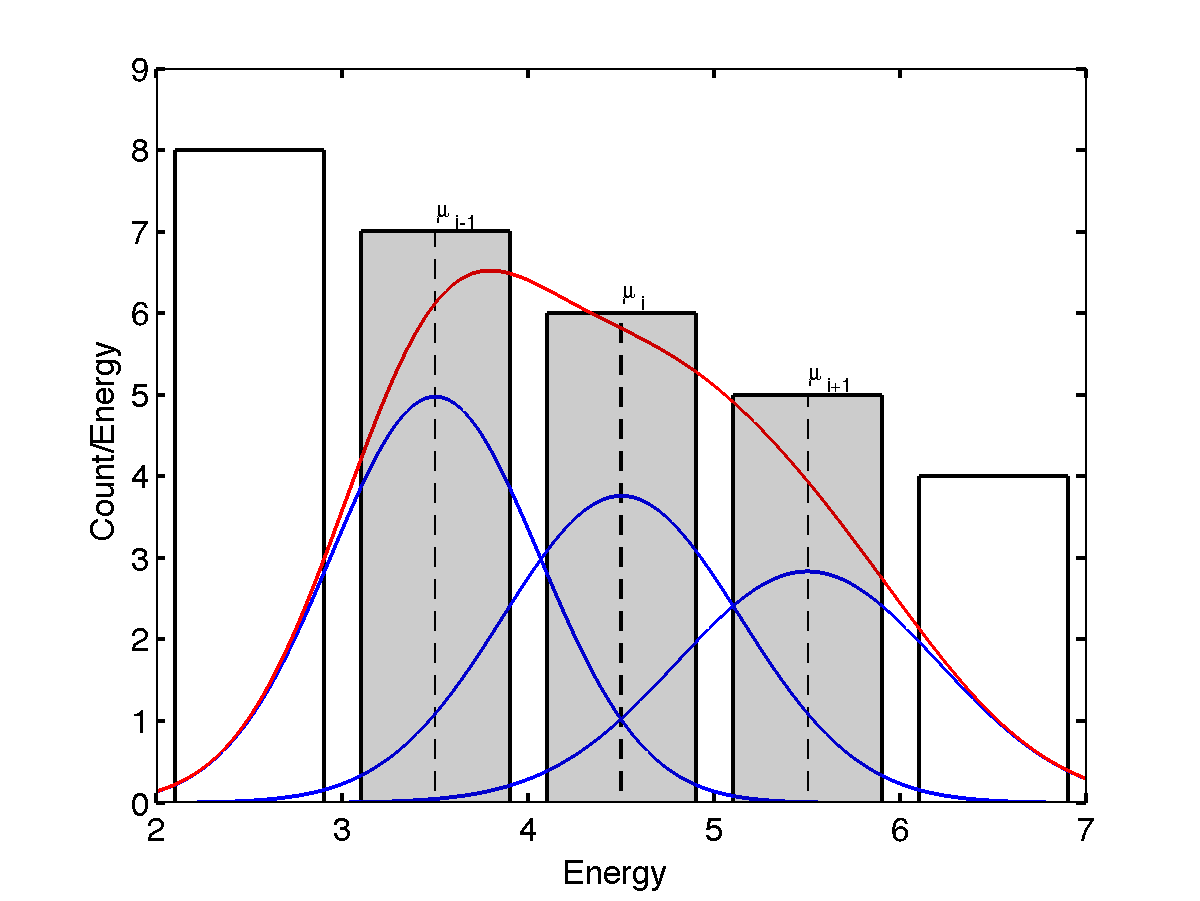
\includegraphics[width=130mm]{Chapter_Flucs/Figures/example_integral}
\caption{}
\label{fig:exp_int}
\end{figure}


\subsection{Calculating the Observed Energy}

After modeling the finite resolution with Gaussians the mean observed at each bin can be calculated from the overlap of all bins weighted by the corresponding means. We can write the observed mean in the $\rm i^{th}$ bin, $\nu_i$, in terms of the bin centers $\mu$ and overlapping areas of all bins using equation \ref{eq:1}:
%\begin{center}
\begin{equation}
\nu_i = \frac{\mathlarger{\sum}\limits_{j=1}^{n}\ \mu_j\mathlarger{\int}\limits_{\mathsmaller{\mu_i-\frac{\Delta x}{2}}}^{\mathsmaller{\mu_i+\frac{\Delta x}{2}}} G_{j}(x)\,\mathrm{d}x} 
{\mathlarger{\sum}\limits_{j=1}^{n} \ \mathlarger{\int}\limits_{\mathsmaller{\mu_i-\frac{\Delta x}{2}}}^{\mathsmaller{\mu_i+\frac{\Delta x}{2}}} G_{j}(x)\,\mathrm{d}x}  
\label{eq:2}
\end{equation}
%\end{center}

Equation \ref{eq:2} can be solved in terms of error function and complimentary error function, first we will generalize a formula to solve for the overlapping area from the $\rm j^{th}$ bin into the $\rm i^{th}$ bin. 
\begin{equation}
%\rm A_i = c_i \ erf\left(\frac{\Delta x}{\sigma_i\sqrt{2}}\right) + \sum\limits_{n\neq i}^{} \frac{c_n}{2} erfc\left(\frac{|\mu_n-\mu_i| - \frac{\Delta x}{2}}{\sigma _n\sqrt{2}} \right) - 
%\sum\limits_{n\neq i}^{} \frac{c_n}{2} erfc\left(\frac{|\mu_n-\mu_i| + \frac{\Delta x}{2}}{\sigma _n\sqrt{2}} \right) 
\rm A_{i,j}=\mathlarger{\int}\limits_{\mathsmaller{\mu_i-\frac{\Delta x}{2}}}^{\mathsmaller{\mu_i+\frac{\Delta x}{2}}}\it G_{j}(x)\,\mathrm{d}x =
\begin{cases}\rm c_i \ erf\left(\frac{\Delta x}{\sigma_i\sqrt{2}}\right), & j=i  \\
\rm \frac{c_j}{2} erfc\left(\frac{|\mu_j-\mu_i| - \frac{\Delta x}{2}}{\sigma _j\sqrt{2}} \right) - 
\rm \frac{c_j}{2} erfc\left(\frac{|\mu_j-\mu_i| + \frac{\Delta x}{2}}{\sigma _j\sqrt{2}} \right) , & j \neq i \end{cases}
\label{eq:3}
\end{equation}

As $\rm \mu$ approaches zero the Gaussian distribution of equation \ref{eq:1} begins to spill over into negative values, which in some cases may be unphysical. For instance, the Gaussian assumption leads to negative photons. We can chose to ignore this area or make the distribution more Poisson like by bouncing the Gaussian back at $\rm \mu = 0$. The formula for accounting for the area of the reflected Gaussian is described in \ref{eq:6}. Ultimately this assumption has little impact on the S1 and S2 analysis because the threshold cut off well before the zero interface is reached, but it does make the distributions more Poisson like near the zeroth bins. Equation \ref{eq:6} is the same as \ref{eq:3} with the bin center $\rm \mu_i$ mapped to $\rm -\mu_i$.

\begin{equation}
%\rm A_i = c_i \ erf\left(\frac{\Delta x}{\sigma_i\sqrt{2}}\right) + \sum\limits_{n\neq i}^{} \frac{c_n}{2} erfc\left(\frac{|\mu_n-\mu_i| - \frac{\Delta x}{2}}{\sigma _n\sqrt{2}} \right) - 
%\sum\limits_{n\neq i}^{} \frac{c_n}{2} erfc\left(\frac{|\mu_n-\mu_i| + \frac{\Delta x}{2}}{\sigma _n\sqrt{2}} \right) 
\rm B_{i,j}=
\rm \frac{c_j}{2} erfc\left(\frac{|\mu_j+\mu_i| - \frac{\Delta x}{2}}{\sigma _j\sqrt{2}} \right) - 
\rm \frac{c_j}{2} erfc\left(\frac{|\mu_j+\mu_i| + \frac{\Delta x}{2}}{\sigma _j\sqrt{2}} \right)
\label{eq:6}
\end{equation}

The error function and complementary error function are defined in equation \ref{eq:4} and the coefficient $\rm c_i$ is defined in equation \ref{eq:1}.
\begin{multline}
\\ \rm erf(x)=\frac{2}{\sqrt{\pi}} \times \int\limits_{0}^{x} exp(-t^2)\\
\rm erfc(x)=\frac{2}{\sqrt{\pi}} \times \int\limits_{x}^{\infty} exp(-t^2) = 1 - erf(x)\\
\label{eq:4}
\end{multline}

Finally, we solve for the observed mean in the $\rm i^{th}$ bin by summing all the Gaussian overlaps $\rm A_{i,j}$ + $\rm B_{i,j}$ (equations \ref{eq:3},\ref{eq:6}), weighting the overlapping area from each bin by the corresponding bin center $\rm \mu_j$. The result is shown in equation \ref{eq:5} and is equivalent to equation \ref{eq:2} when the area from the reflected Gaussian is not considered, $\rm B_{i,j}$=0.
\begin{equation}
\rm \nu_i =  \frac{\sum\limits_{j=1}^{n}\mu_j\cdot (A_{i,j}+B_{i,j})}{\sum\limits_{j=1}^{n} (A_{i,j}+B_{i,j})}
\label{eq:5}
\end{equation}

\subsection{Smearing a Toy Spectrum}

To demonstrate the application of equation \ref{eq:5} we use it to smear a toy linearly decaying spectrum. By modifying the dependence of $\rm \sigma_i$ on $\rm \mu_i$ we can better understand the effects of the spectral shape and the functional for of the resolution.

Figure \ref{fig:Toy_Linear} shows the effect of the finite resolution on a linearly decaying spectral shape. Using a constant resolution $\rm \sigma$ the observed mean, when accounting for finite resolution, shifts down due to the spectral shape. In the case with $\rm \sigma_i \sim \sqrt{\mu_i} $ the observed mean at first shifts higher as the increasing width at higher value bin centers, even with lower counts, out weighs the lower bin centers with higher counts and narrower widths. In both cases as the bin centers approach zero the observed mean shifts higher due to an imposed threshold at zero, here Poisson statistics take over and the Gaussian characterization leads to a loss of events below zero. Thus, for the sake of the toy model in figure \ref{fig:Toy_Linear} we only characterize the relation between the real mean and the observed mean from the second bin center. It is also worth mentioning that for the case of having a varying resolution in figure \ref{fig:Toy_Linear} the shift in spectral shape seems minor, yet there is a a significant 20\% deviation in the observed mean of the last bin.

 \begin{figure}[h!]\centering
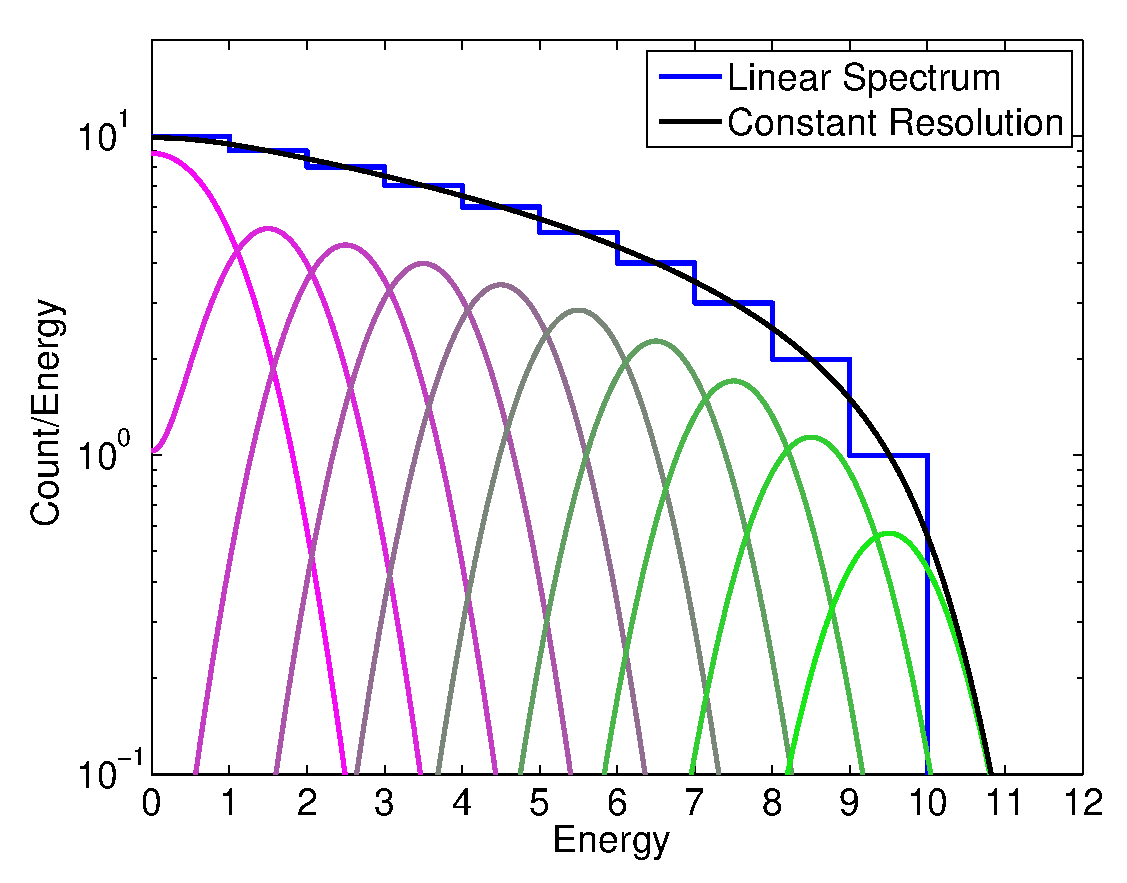
\includegraphics[width=70mm]{Chapter_Flucs/Figures/Toy_Model_lin_const}
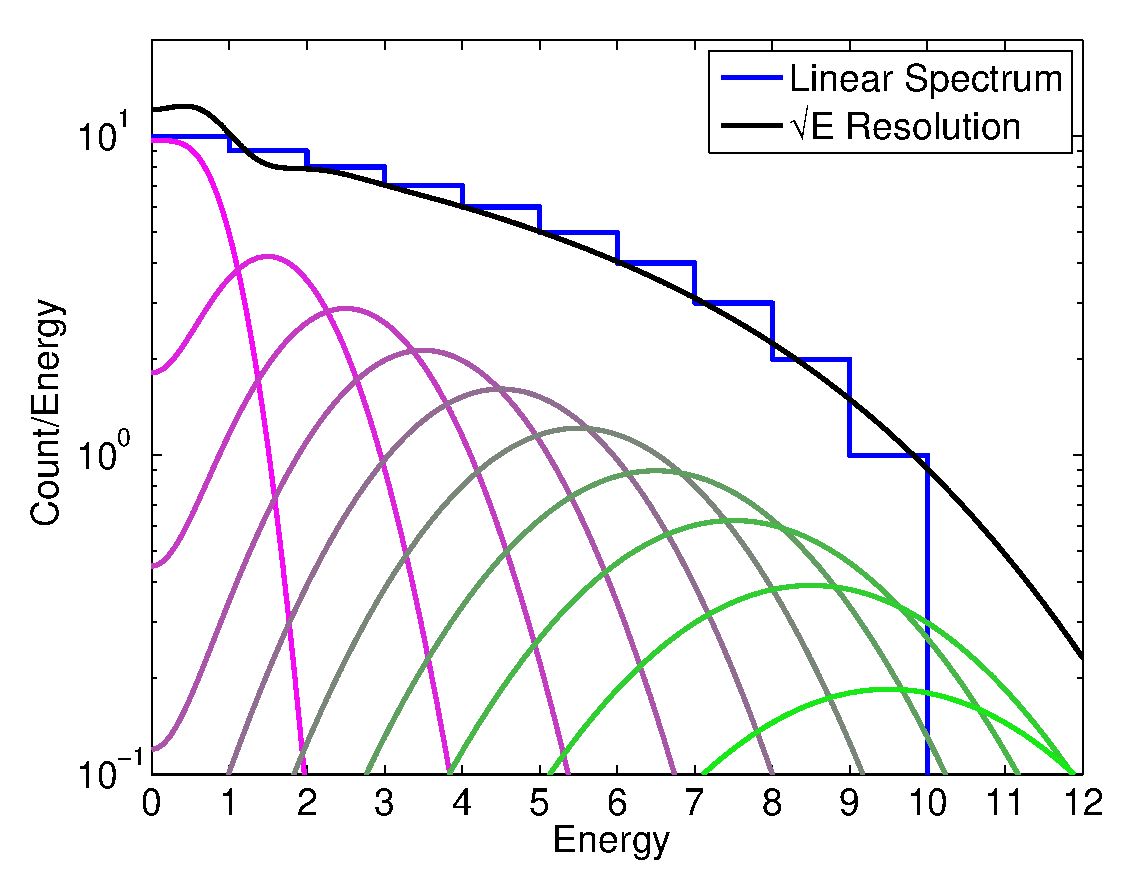
\includegraphics[width=70mm]{Chapter_Flucs/Figures/Toy_Model_lin_dep}
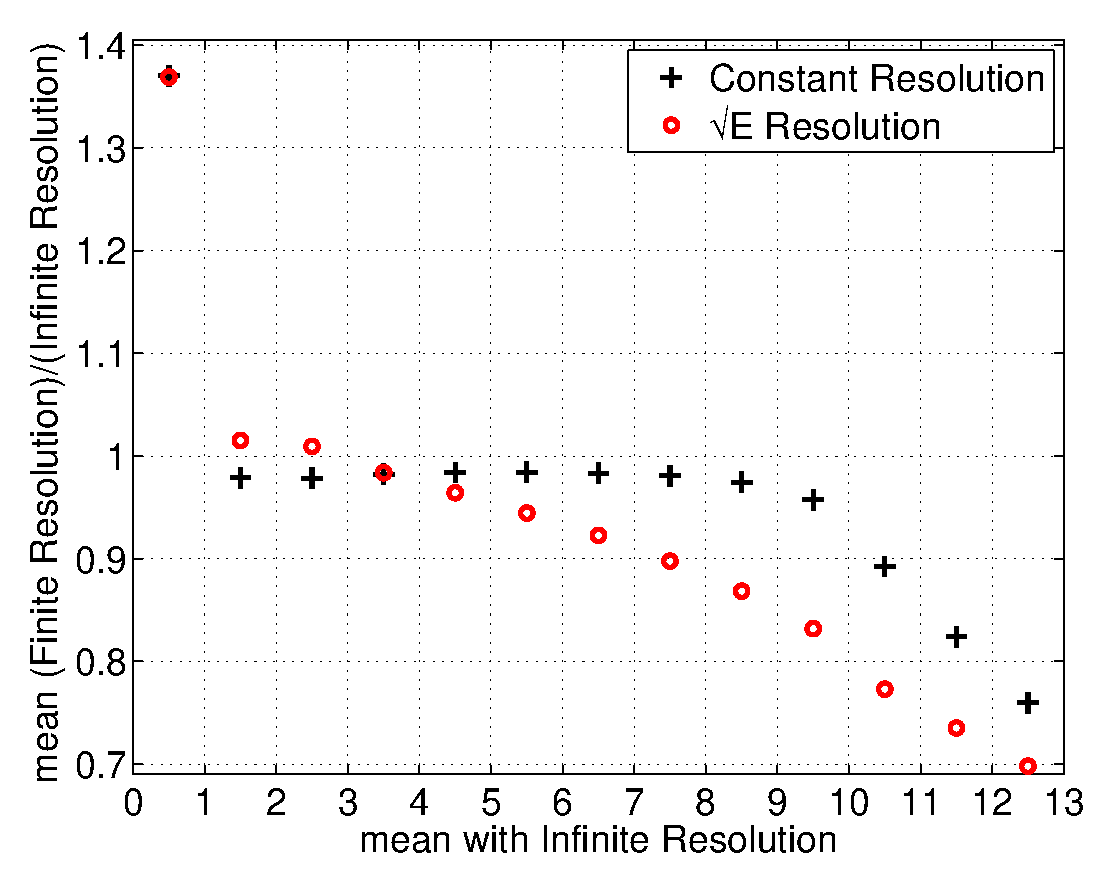
\includegraphics[width=70mm]{Chapter_Flucs/Figures/Toy_Model_mean_shift}
\caption{Top Left: A linearly decaying spectrum, in blue. The black curve represents the sum of the Gaussians assuming a constant resolution. Top Right: A linearly decaying spectrum, in blue. The black curve represents the sum of the Gaussians with a $\rm \sqrt{E}$ dependent resolution. Bottom: The observed mean, with finite resolution, compared to the real mean with infinite resolution. The black points are for the case with linear resolution and the red points represent the case with $\rm \sqrt{E}$ dependent resolution.}
\label{fig:Toy_Linear}
\end{figure}

\newpage



\section{LY, QY and NEST}

The first attempt to undue the effect of the tritium spectral shape and finite detector resolution is to use the NEST model \cite{NEST_2013}. We take the light yield (LY) and charge yields (QY) from the NEST model and convolve it with the known tritium energy spectrum to produce the S1 and S2 spectra. The S1 and S2 spectra are then smeared with detector resolution and recombination fluctuations, determined in chapter \ref{Ch:ch4}. It is found  that the S1 and S2 spectra from the data deviate from the NEST model making it difficult to reverse engineer the effect of smearing. However, taking the NEST model to be correct within 20\% the spectral shape correction is calculated and found to be small. We proceed to extract LY, QY and $\rm \sigma R$ from the tritium data without any correction, producing a model that is more accurate than NEST (which has yet to be vetted at our electric field and energy). The LY, QY and  $\rm \sigma R$ can then be convolved with the true tritium energy spectrum and detector resolution in order to calculate a more accurate spectral shape correction.

%The first step is to solve for the value of $\rm \sigma_R$ (recombination fluctuation) that needs to be input into the smearing model, the statistical part from detector resolution remains fixed. Figure \ref{fig:R_T} show the optimal value of $\rm \sigma_R$ being extracted from the tritium data, starting with an initial guess based on the recombination fluctuation measured from the $\rm^{83m}Kr$ data.


\subsection{Tritium S1 and S2 Mean and NEST}

The spectral shape correction for the mean of the observed S1 and S2 signal from tritium beta decay can be solved for using equation \ref{eq:5}. We start with NEST to get the expected S1 and S2 tritium spectrum and applying equations \ref{eq:1}-\ref{eq:5} to map the observed mean to the true mean. The resolution of S1 and S2 arise from recombination, statistical and instrumental fluctuations and is given in equation \ref{eq:SigStat} and \ref{eq:SigInst}. We use equations \ref{eq:S1_res} and \ref{eq:S2_res} to smear the photon and electron yields from NEST, simulating detector resolution. The use of Gaussian sigma down to low S1 is an acceptable approximation since underlying distribution actually consists of the number of photons, $\rm n_\gamma = \frac{S1}{g1}$. With g1=0.097 there are still 30 photons near the S1 threshold of 3 PE. The S2 threshold is around 300 PE, $\rm n_e = \frac{S2}{g2}$. With g2=5.75 there are still 50 electrons near end of the tritium spectrum.

%We will use the Gaussian approximation as it makes the application of equations \ref{eq:1}-\ref{eq:5} simpler.
%The variance in S1 due to recombination fluctuations, statistical fluctuations and instrumental fluctuations at a given energy. The functional form of all three have been previously measured and can be extrapolated for use with the tritium spectrum. The first step is to use the expected light yields from NEST along with the measured smearing from recombination and detector resolution to extract a correction factor for the observed S1 signal. Having a priori knowledge of light yields will allow for the spectral shape to be corrected or can at least be used to approximate an error when we go to extract the light yield and recombination fluctuations from the tritium beta spectrum.

\begin{equation}
 \rm \sigma_{S1}^2=g_1^2(\sigma_{n_{\gamma_{stat}}}^2+\sigma_{n_{\gamma_{inst}}}^2+\sigma_R^2)
\label{eq:S1_res}
\end{equation}

\begin{equation}
 \rm \sigma_{S2}^2=g_2^2(\sigma_{n_{e_{stat}}}^2+\sigma_{n_{e_{inst}}}^2+\sigma_R^2)
\label{eq:S2_res}
\end{equation}


%The correction is calculated starring with the NEST photon and electrons yields \cite{NEST_2013}, applying the gain g1 or g2, and convolving it with a tritium beta spectrum along with our approximation of recombination fluctuations measured in equation \ref{eq:Inst_Fit}. 

Figure \ref{fig:S1S2_mapping} (a,c) shows the application of smearing from equation \ref{eq:S1_res} and \ref{eq:S2_res} to the expected S1 and S2 tritium spectrum, respectively, overlaid with the data. The mapping of the observed S1 and S2 to the real S1 and S2 is shown in \ref{fig:S1S2_mapping} (b,d). The mapping is the result of taking the fit for detector resolution vs. the number of photons and electrons in equation \ref{eq:SigDet} we apply the model as outlined in \ref{sec:Smear} to calculate the shift from observed mean photons to real mean. %Applying the correction factor to the data reveals the mean S1s that the LUX detector would observe given infinite detector resolution.

% S1 S2 result NEST iter 0
\renewcommand{\baselinestretch}{1}
\small\normalsize
\begin{figure}[h!]\centering
 
\subcaptionbox{S1 \label{fig:5a}}{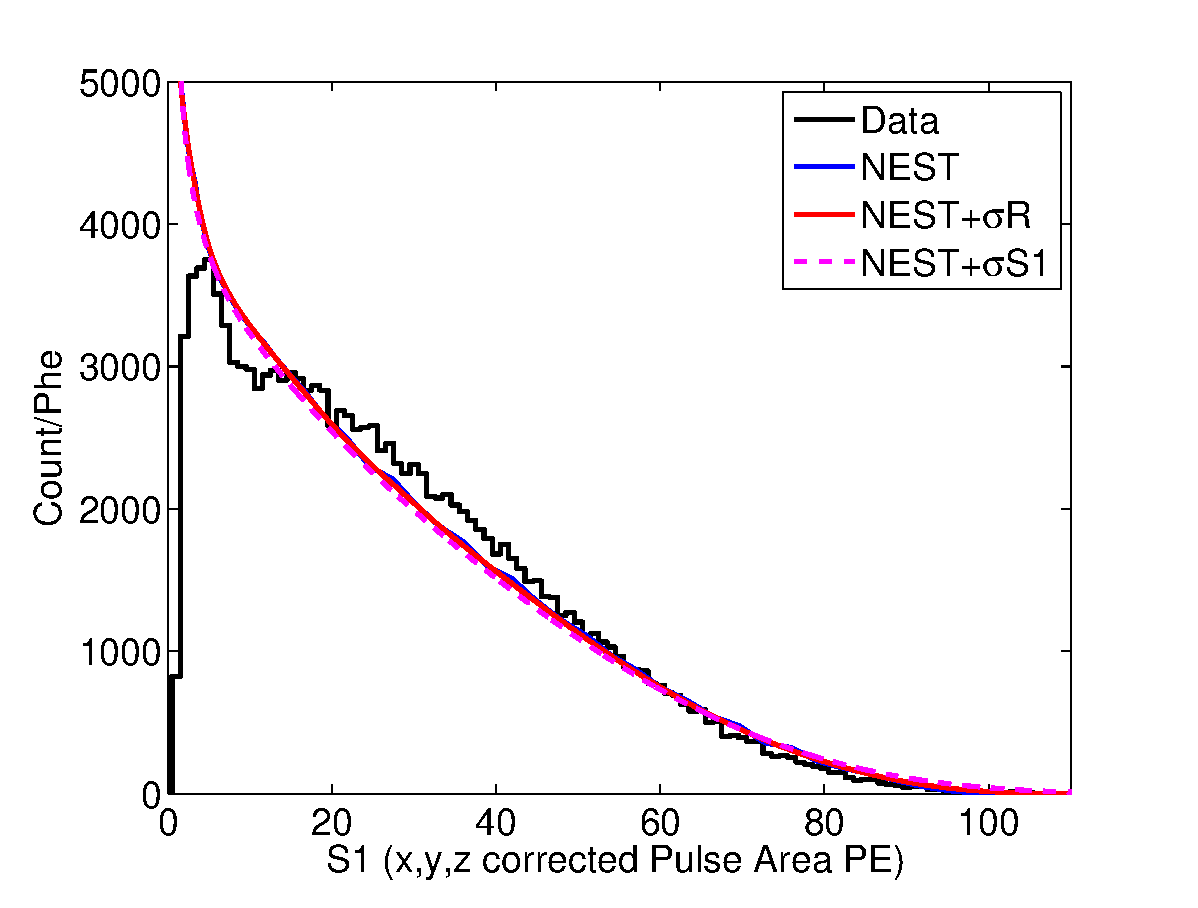
\includegraphics[width=73mm]{Chapter_Flucs/Figures/S1S2_Spectra/S1_spec_compare_.eps}}
\hfill
\subcaptionbox{S1 \label{fig:5b}}{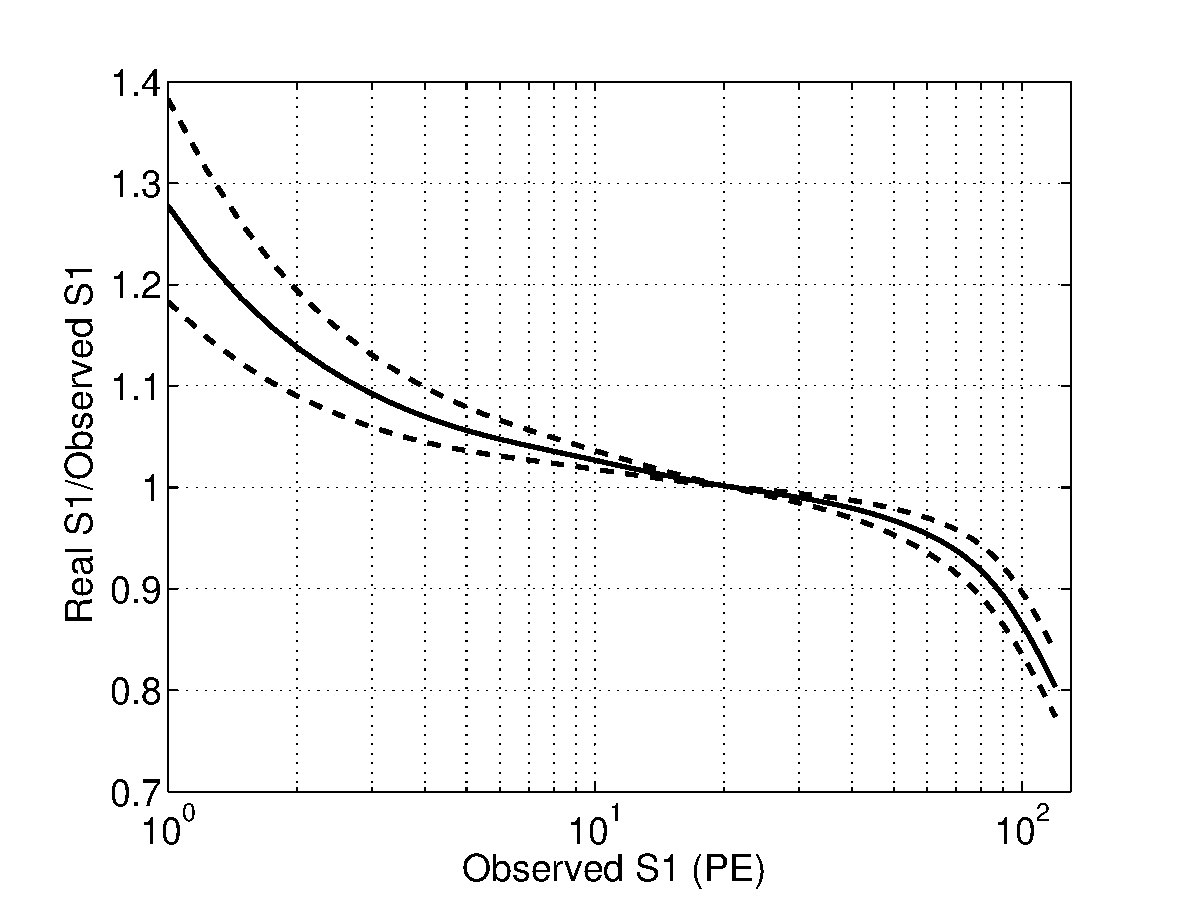
\includegraphics[width=73mm]{Chapter_Flucs/Figures/S1S2_Spectra/S1_corr_.eps}}

\bigskip

\subcaptionbox{S2 \label{fig:5c}}{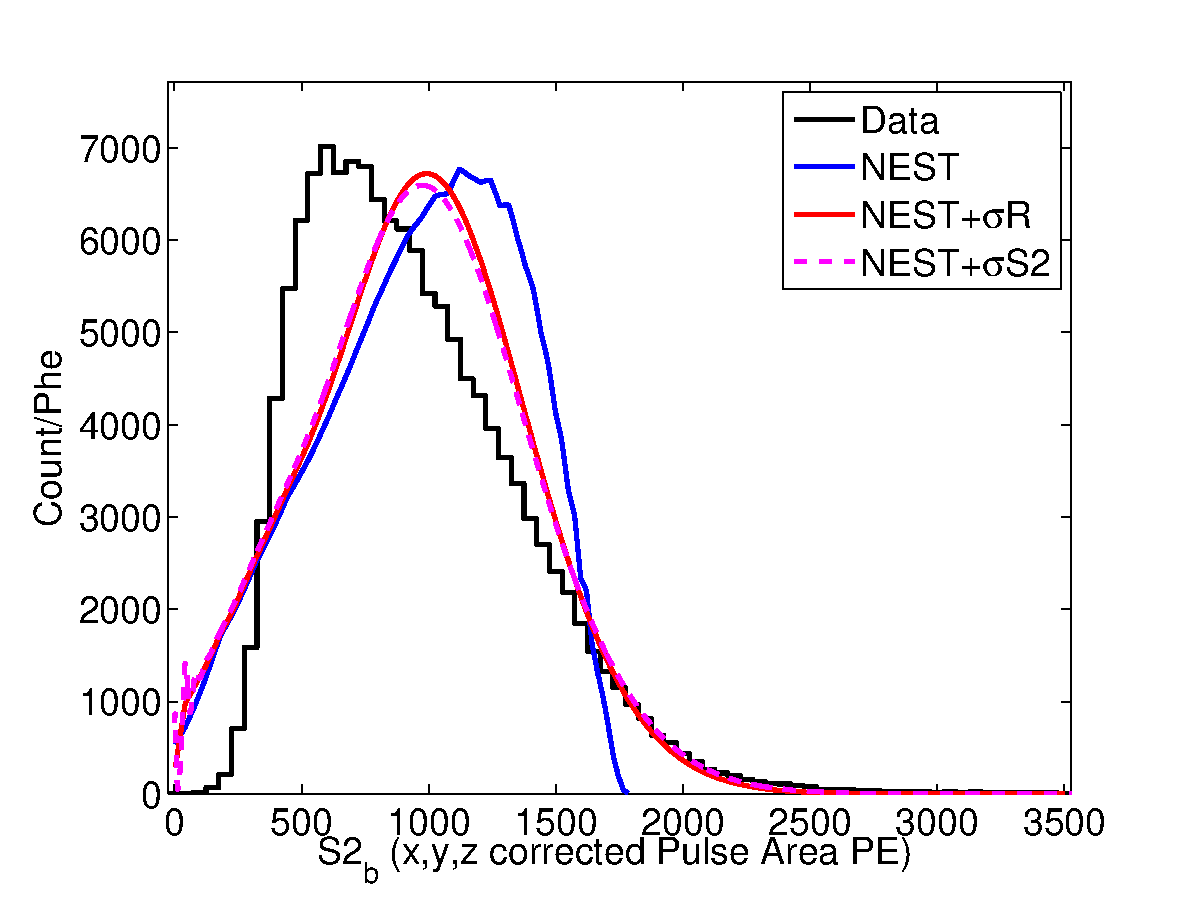
\includegraphics[width=73mm]{Chapter_Flucs/Figures/S1S2_Spectra/S2_spec_.eps}}
\hfill
\subcaptionbox{S2 \label{fig:5c}}{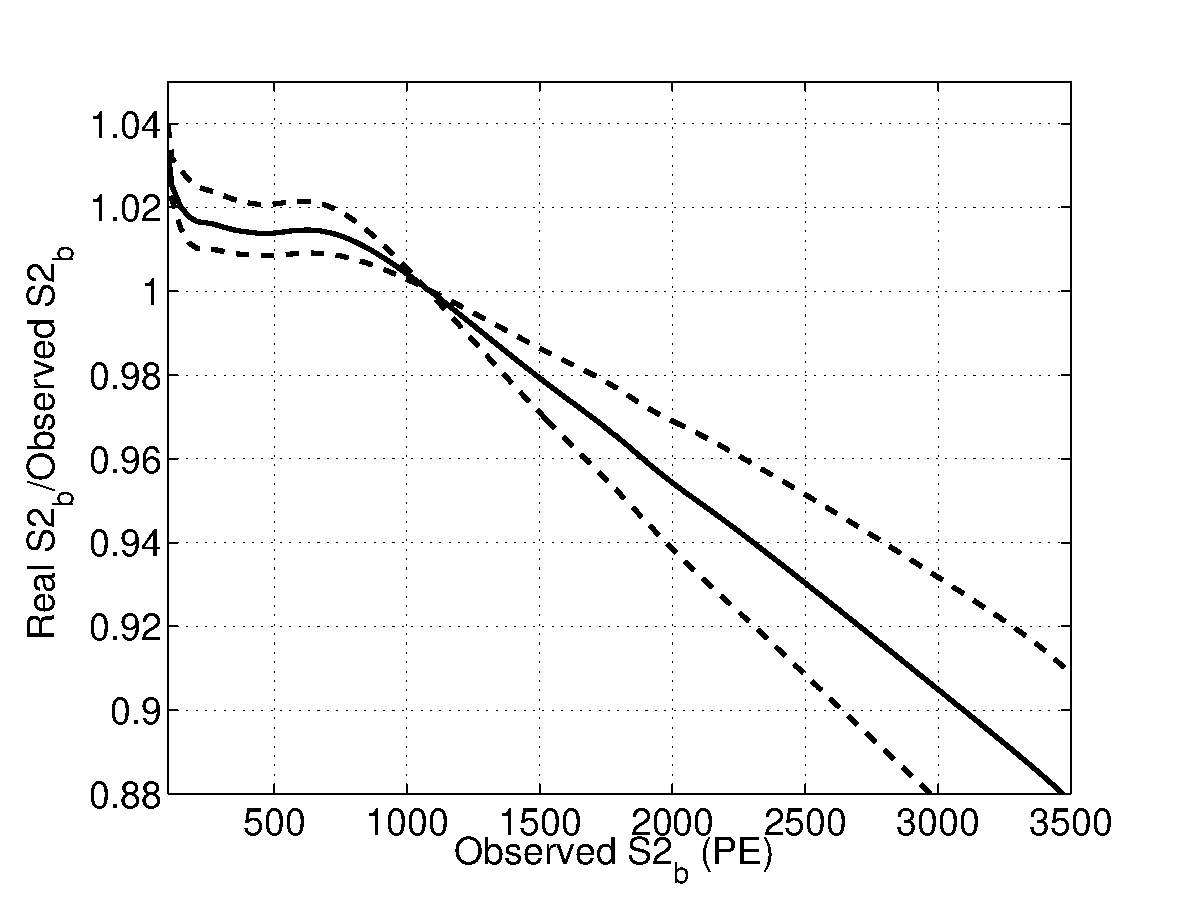
\includegraphics[width=73mm]{Chapter_Flucs/Figures/S1S2_Spectra/S2_corr_.eps}}

\caption{ a): In Black S1 tritium spectrum extracted from the data. In blue, The NEST light yield curve. In red, the NEST light yield curve with recombination fluctuations. Dashed magenta is NEST light yield with smearing from equations \ref{eq:S1_res}.  b): The ratio of the real mean to the observed mean vs. the observed mean for a tritium photon spectrum. Note the S1 threshold at about 3 Phe in S1. c): In Black S2 tritium spectrum extracted from the data. In blue, The NEST light yield curve. In red, the NEST light yield curve with recombination fluctuations. Dashed magenta is NEST light yield with smearing from equations \ref{eq:S2_res}.  d): The ratio of the real mean to the observed mean vs. the observed mean for a tritium photon spectrum. Note the S2 threshold at about 400 Phe in S2. }

\label{fig:S1S2_mapping}
\end{figure}
\renewcommand{\baselinestretch}{2}
\small\normalsize


We find that that S1and S2 spectra deviate from the data by up to 20\%. The deviation is especially evident from the S2 spectrum for which the peak is ~20\% off from the NEST charge yield model. These discrepancies maybe arising from the error of error in g1 and g2 which could systematically shift light yield and charge yield by the appropriate amount. However, modifying g1 and g2 only induces a horizontal shift left or right where the S1 spectrum indicates the need to modify the derivative of LY and QY from NEST



\begin{comment}
 \begin{figure}[h!]\centering
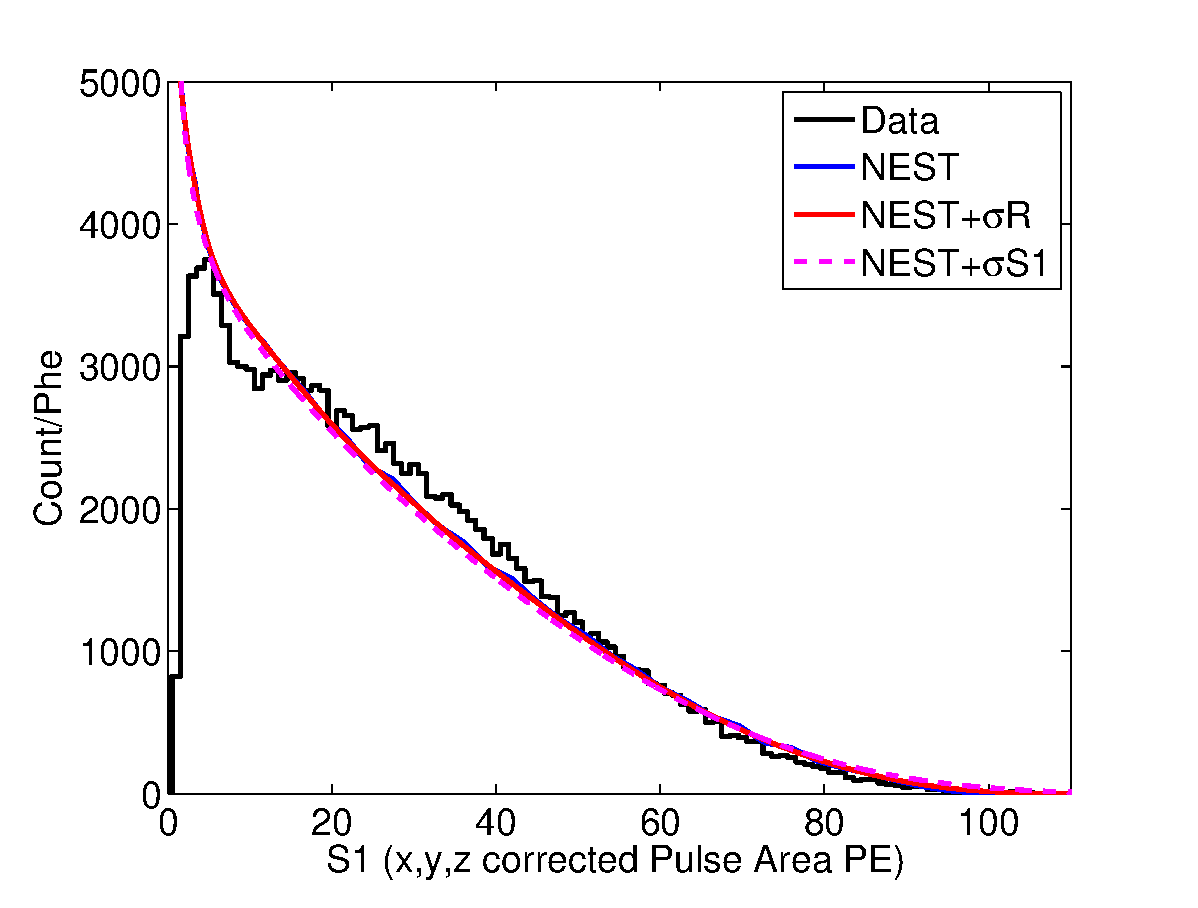
\includegraphics[width=70mm]{Chapter_Flucs/Figures/S1S2_Spectra/S1_spec_compare_.eps}
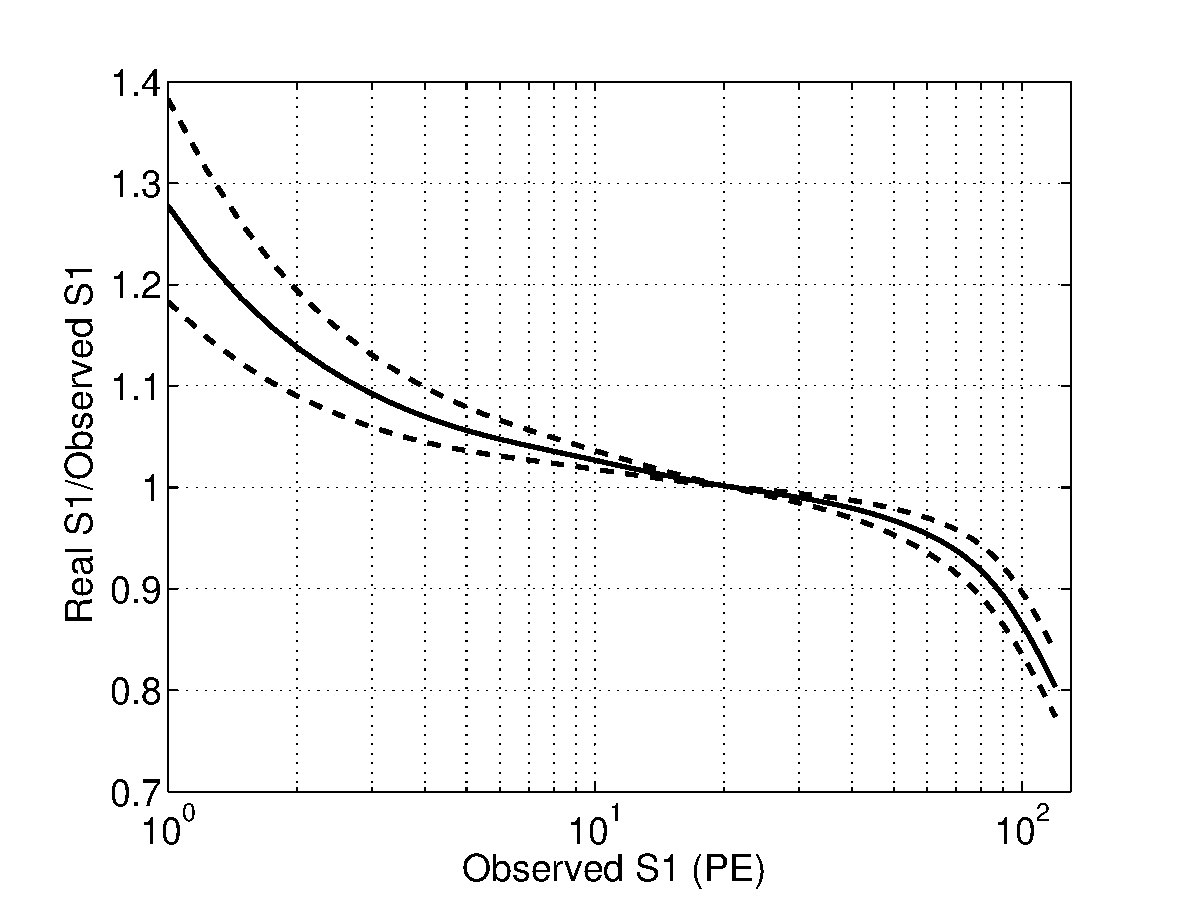
\includegraphics[width=70mm]{Chapter_Flucs/Figures/S1S2_Spectra/S1_corr_.eps}
\caption{Left: In Black S1 tritium spectrum extracted from the data. In blue, The NEST light yield curve. In red, the NEST light yield curve with recombination fluctuations. Dashed magenta is NEST light yield with smearing from equations \ref{eq:S1_res}.  Right: The ratio of the real mean to the observed mean vs. the observed mean for a tritium photon spectrum. Note the S1 threshold at about 3 Phe in S1. }
\label{fig:S1_mapping}
\end{figure}

 \begin{figure}[h!]\centering
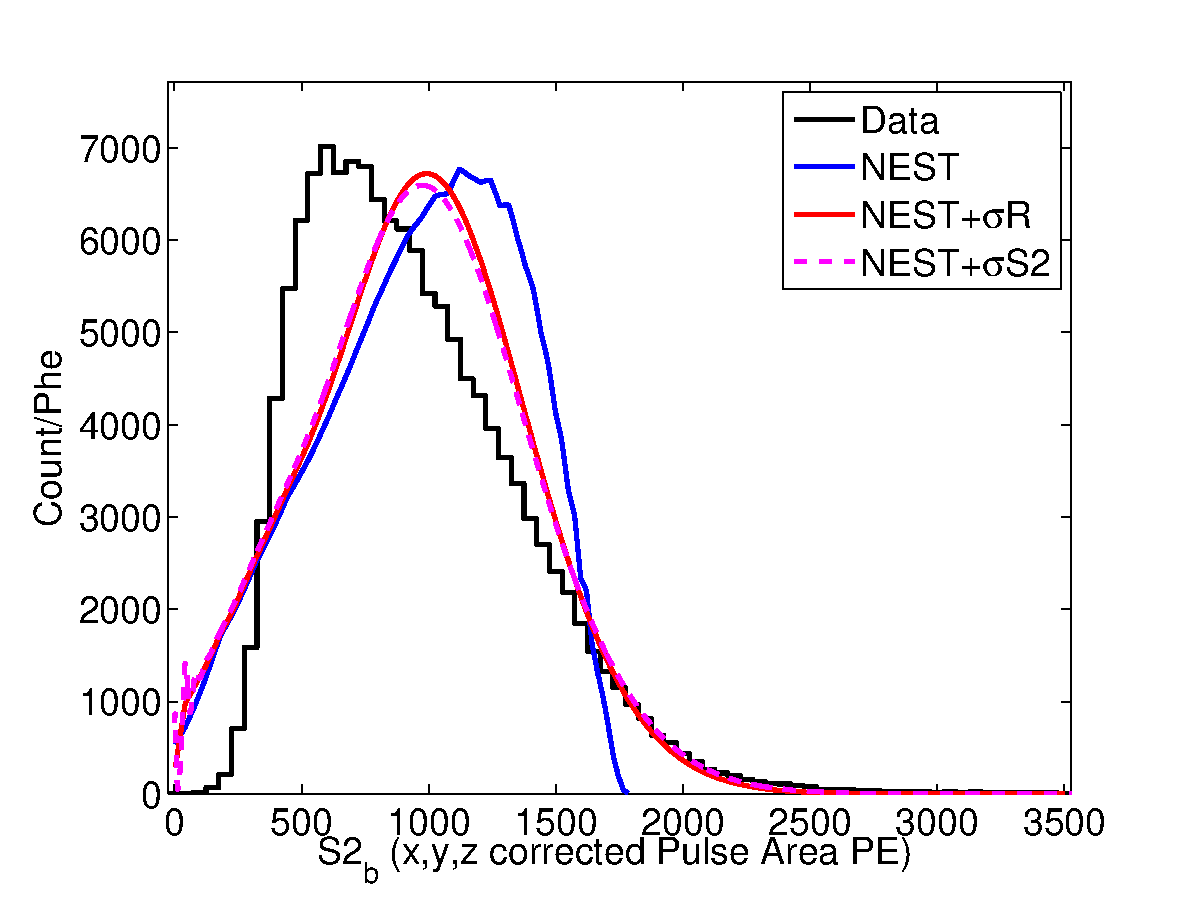
\includegraphics[width=70mm]{Chapter_Flucs/Figures/S1S2_Spectra/S2_spec_.eps}
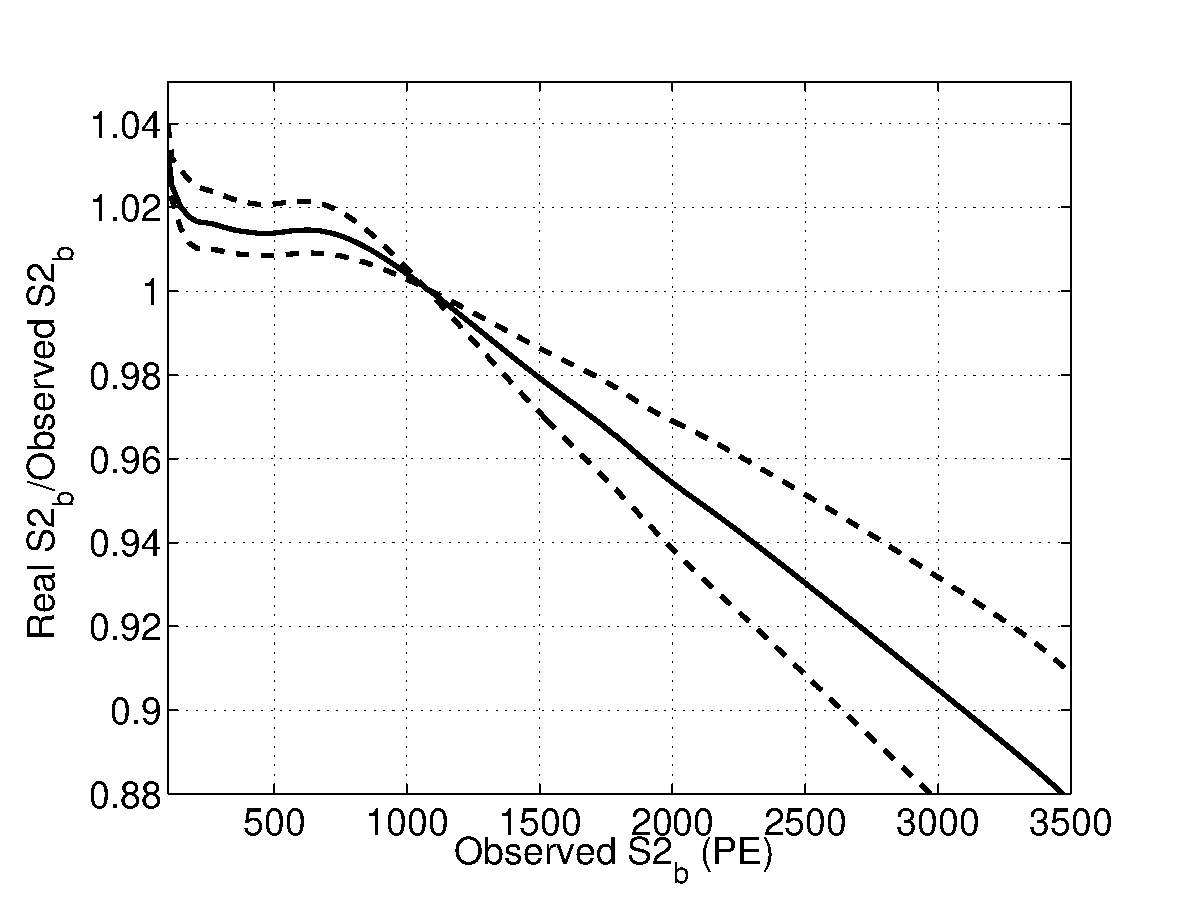
\includegraphics[width=70mm]{Chapter_Flucs/Figures/S1S2_Spectra/S2_corr_.eps}
\caption{Left: In Black S2 tritium spectrum extracted from the data. In blue, The NEST light yield curve. In red, the NEST light yield curve with recombination fluctuations. Dashed magenta is NEST light yield with smearing from equations \ref{eq:S2_res}.  Right: The ratio of the real mean to the observed mean vs. the observed mean for a tritium photon spectrum. Note the S2 threshold at about 400 Phe in S2. }
\label{fig:S2_mapping}
\end{figure}
\end{comment}

%\subsection{Tritium S2 Mean and NEST}

%The correction for the mean of the measured charge yield, S2 PE, for tritium beta decay can be solved for using equation \ref{eq:5}. Starting with a simulated S2 tritium spectrum with infinite resolution and applying equations \ref{eq:1}-\ref{eq:5} one can attain the mapping of measured mean to true mean.  The resolution of S2 was determined from statistical and  instrumental fluctuations and is given in equation \ref{eq:SigStat} and \ref{eq:SigInst}. The use of Gaussian error down to low S2 is an acceptable approximation since the S2 spectrum ends at 300 PE, $\rm n_e = \frac{S2}{g2}$. With g2=5.75 there are still 50 electrons near end of the tritium spectrum, thus the Gaussian model is still a close approximation of the underlying Poisson distribution. We will use the Gaussian approximation as it makes the application of equations \ref{eq:1}-\ref{eq:5} much simpler.
%As in the case of the light yield, the variance in S2 is the result of recombination fluctuations, statistical fluctuations and instrumental fluctuations at a given energy. The functional form of all three have been previously measured and can be extrapolated for use with the tritium spectrum. We first use the expected charge yields from NEST along with the measured smearing from recombination and detector resolution to extract a correction factor for the observed S2 signal. Having a priori knowledge of light yields will allow for the spectral shape to be corrected or can at least be used to approximate an error when we go to extract the charge yield and recombination fluctuations  from the tritium beta spectrum.






\subsection{Tritium Energy Spectrum}

The mapping of the observed energy to real energy was determined using a full simulation of tritium beta decay. The accuracy of the smearing model described in equations \ref{eq:1}-\ref{eq:5} can be tested by comparing it against the energy observed after a full NEST simulation. The energy depends on both S1 and S2 thus, mapping observed energy to true energy my be non trivial. Again, we start with a simulated tritium energy spectrum with infinite resolution and apply the empirically determined resolution in equation \ref{eq:E_res}, measured with $\rm^{127}Xe$ X-rays and $\rm ^{83m}Kr$ calibrations. Figure \ref{fig:E_spec} shows the comparison of smearing model vs true energy along with the smearing after running full photon and electron propagation in LUXSIM vs the true energy. The smearing form the model described in equations \ref{eq:1}-\ref{eq:5} is almost identical to the output of LUXSIM. The energy spectrum flares out at low energy, is pulled in from 5-10 [keV] and again flares out slightly above 15 [keV]. It is important to note that the change in the spectral shape is hardly noticeable, as was the case with S1 and somewhat with S2. Figure \ref{fig:E_mapping} shows the results for mapping observed energy to real energy using both smearing methods. The two methods show good agreement down to the threshold of 1.5 [keV], the agreement with simulation is always within 1\%. Below 2 [keV] the model predicts the ratio of true energy to observed energy to rise as there are greater number of events at higher energy spilling over to lower energy, the simulation however does not show this behavior leading to a 5\% discrepancy in the 1 [keV] bin. We take the difference between the smearing model and LUXSIM as a systematic uncertainty. 

Using equation \ref{eq:Fano}, \ref{eq:Gain} and \ref{eq:E_res1} we solve for the the spread in E as a function energy \ref{eq:E_res}. $\rm a_\gamma$ and $\rm a_e$ are the coefficients in front of the root n term on the $\rm n_\gamma$ and $\rm n_e$ statistical variance . W=73 [$\rm \frac{N_{quanta}}{keV}$].

\begin{gather}
\label{eq:E_res1} \rm E= \frac{1}{W}(n_\gamma + n_{e^-}) \\
 \rm \sigma E^2= \frac{1}{W^2}(\sigma n_\gamma ^2 + \sigma n_{e^-} ^2)\\ 
 \rm \sigma E^2= \frac{1}{W^2}(a_\gamma^2 n_\gamma + a_e^2 n_{e^-})\\
 \rm \sigma E^2= \frac{(a_\gamma+a_e)^2}{W}\frac{(n_\gamma + n_{e^-})}{W}\\
 \rm \sigma E^2= \frac{(a_\gamma+a_e)^2}{W}E\\
  \rm \sigma E= \frac{(a_\gamma+a_e)}{\sqrt{W}}\sqrt{E}
\label{eq:E_res}
\end{gather}

\newpage

 \begin{figure}[h!]\centering
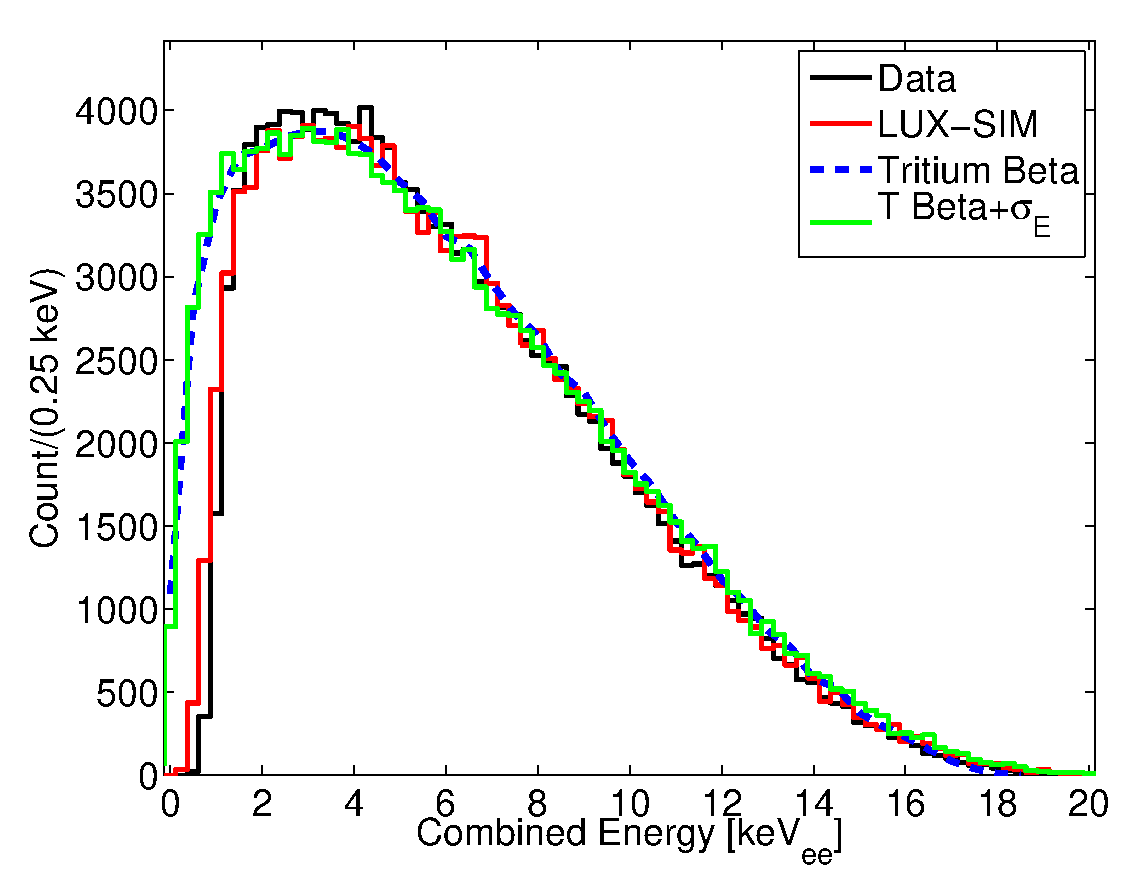
\includegraphics[width=70mm]{Chapter_Flucs/Figures/E_Spec/E_spec_compare_SIM.eps}
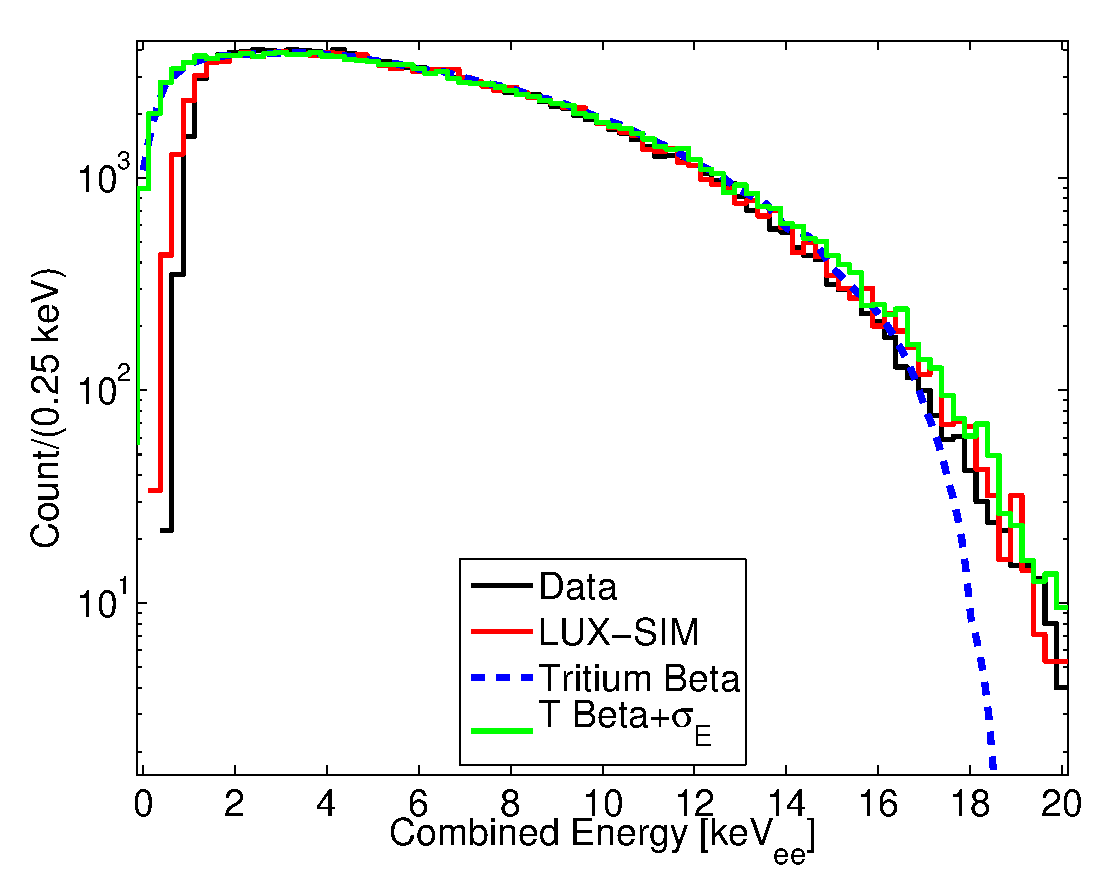
\includegraphics[width=70mm]{Chapter_Flucs/Figures/E_Spec/E_spec_compare_SIM_log_.eps}
\caption{The tritium energy spectrum reconstructed from the data using both Pulse Area and Spike count for S1. Along with LUX SIM, the true tritium beta spectrum and a tritium spectrum smeared with detector resolution. }
\label{fig:E_spec}
\end{figure}


 \begin{figure}[h!]\centering
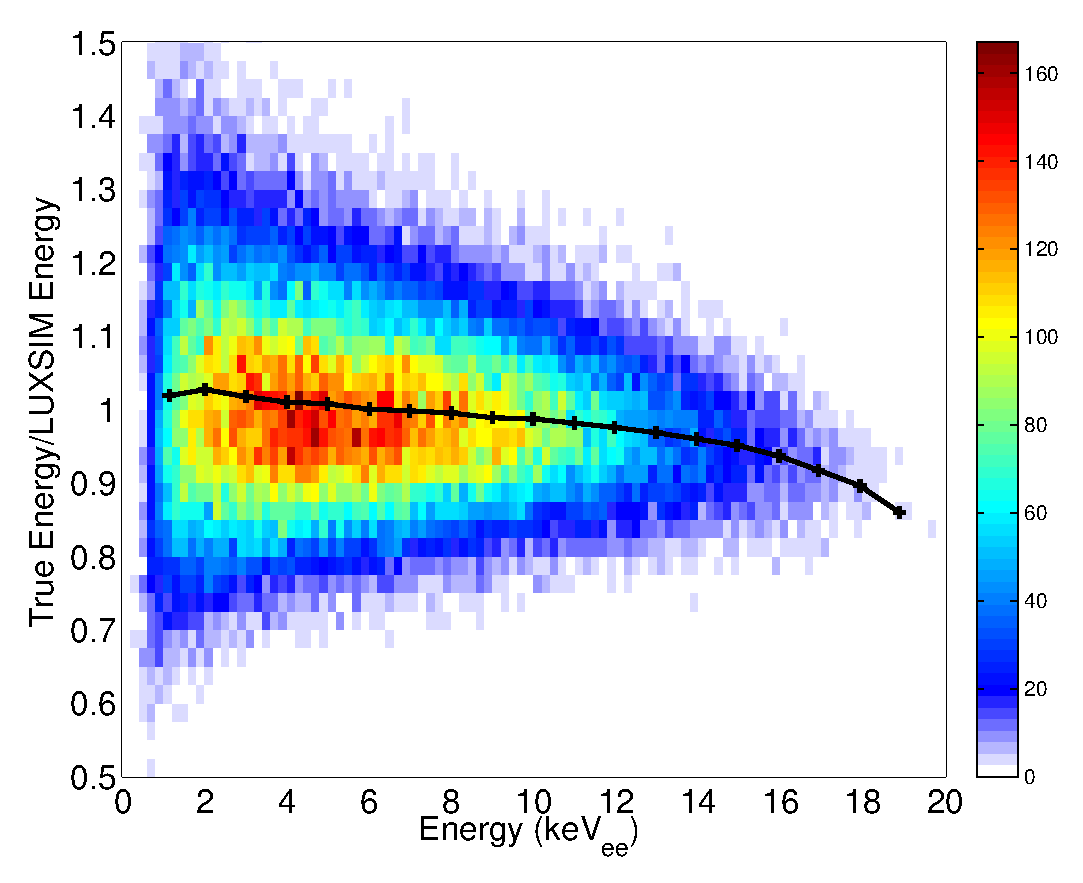
\includegraphics[width=70mm]{Chapter_Flucs/Figures/E_density_LUX_SIM_Tritium.eps}
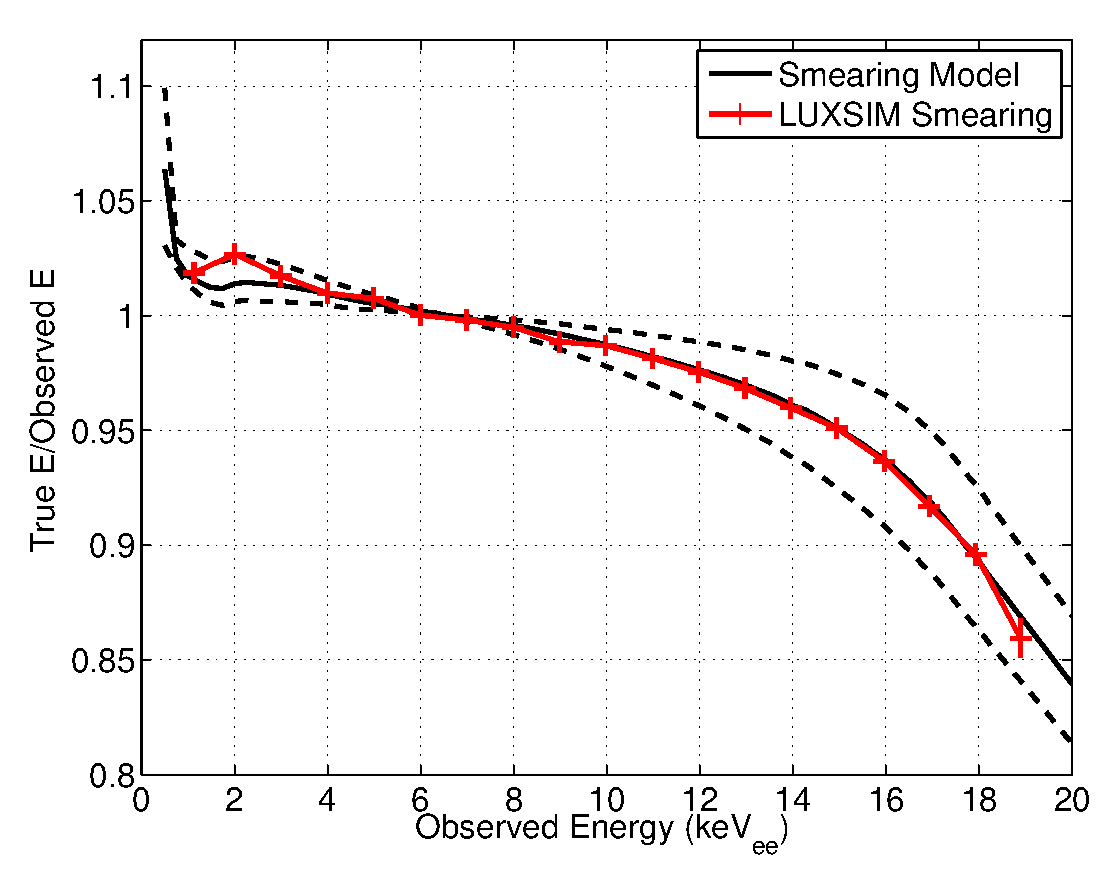
\includegraphics[width=70mm]{Chapter_Flucs/Figures/E_corr.eps}
\caption{Left, mapping from real Monte Carlo energy to observed energy after applying a finite resolution using LUXSIM. Right, comparing the correction determined from the Monte Carlo (Red) to the detector smearing model (black) given in equation \ref{eq:E_res}. The dashed lines represent the uncertainty in the measured value of F(E). The agreement is within errors from 1 to 18 keVee. The Energy threshold is near 1.0 $\rm keV_{ee}$.}
\label{fig:E_mapping}
\end{figure}



\subsection{LY, QY, $\rm \sigma R$ Result}

 The S1 and S2 spectral shape is not a good match with the light yield model from NEST, thus applying a correction to the observed means using NEST is not prudent. Fortunately, we see that both in the S1 and S2 region of interest were the majority of the tritium events occur the spectral shape correction is less than 10\%. Further, the reconstructed energy, uncorrected for spectral shape, is go to within 10\% as well. Knowing this we can move forward with extracting a more accurate light yield and recombination fluctuation accepting the small error in order to create a more accurate model than NEST to which then we can apply the spectral shape correction.

\begin{comment} % skip this part. alread discussed recombination fluctuations.
\newpage 

 \begin{figure}[h!]\centering
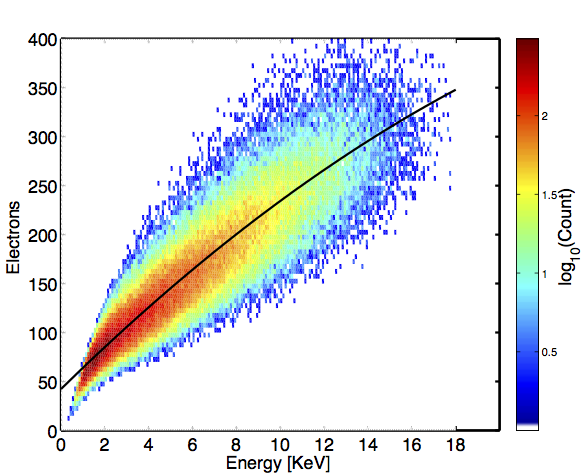
\includegraphics[width=70mm]{Chapter_Flucs/Figures/Iter0/n_electron_180_LY_QY_0.png}
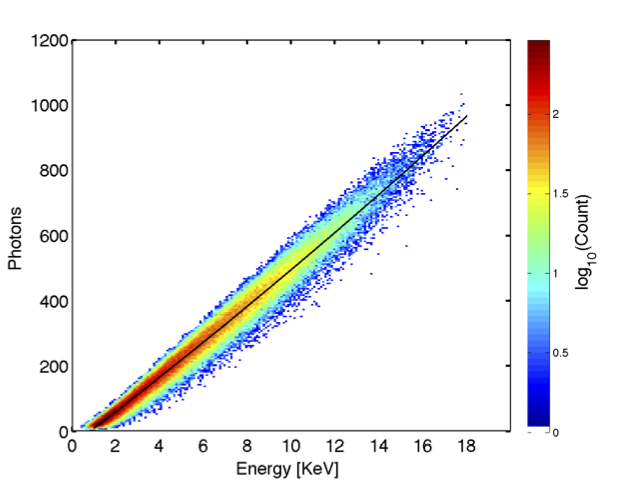
\includegraphics[width=70mm]{Chapter_Flucs/Figures/Iter0/n_photon_180_LY_QY_0.png}
\caption{Number of photons (left) and electrons (right) vs. energy from tritium data without spectral shape correction. The spread in quanta per energy bin is used to measure recombination fluctuations.}
\label{fig:LYQY_0}
\end{figure}

 \begin{figure}[h!]\centering
 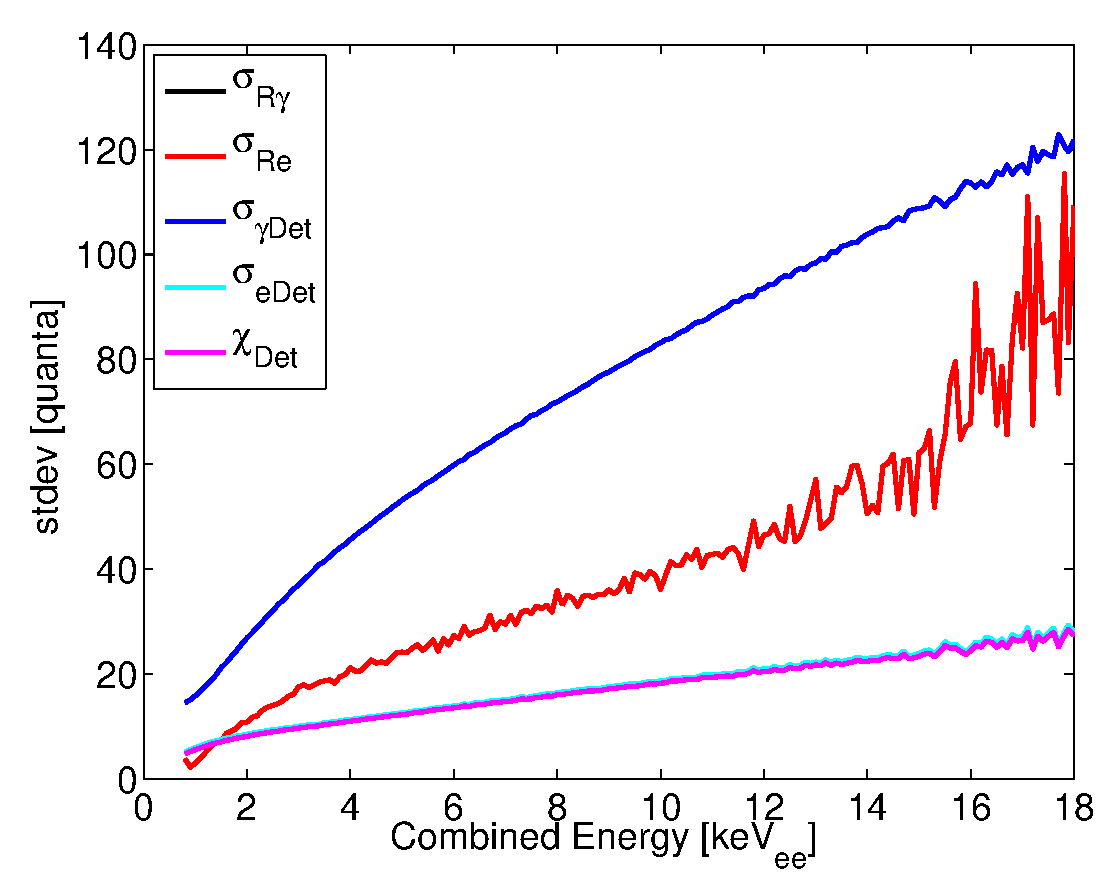
\includegraphics[width=90mm]{Chapter_Flucs/Figures/Iter0/std_fig_.eps}
 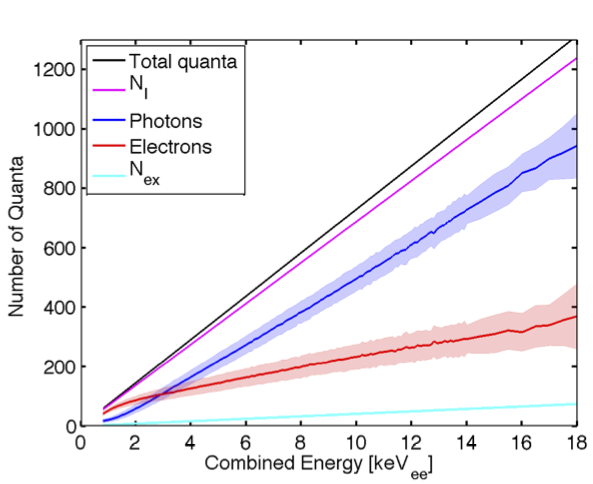
\includegraphics[width=72mm]{Chapter_Flucs/Figures/Iter0/quanta_LY_QY_0.png}
 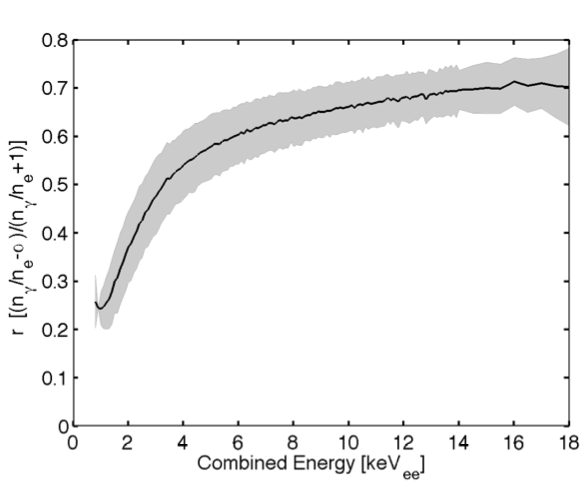
\includegraphics[width=72mm]{Chapter_Flucs/Figures/Iter0/R_LY_QY_0.png}
\caption{Top: Extracted recombination fluctuation from the tritium data from fluctuations in photons and electrons (Black and Red receptively). Bottom right: mean number of quanta in photons, electrons, ions, exitons vs. energy [keV] for the tritium calibrations. Bottom left: Recombination fraction and the one sigma (shaded) vs. energy [keV].}
\label{fig:Rec_0}
\end{figure}

Having extracted light yield (Photons/keV] and charge yield (electrons/keV) we compare the initial result from the tritium data to NEST, and is shown in figure \ref{fig:LYQY_0}. The disagreement between the data and the NEST yields was expected since previously the S1 and S2 tritium spectrum did not line up, in the previous section. Though the means do not match the measured light yield is within 1 sigma considering the large error in gains g1 and g2.

\end{comment}
%LY QY result iter 0

\renewcommand{\baselinestretch}{1}
\small\normalsize
\begin{figure}[h!]\centering
 
\subcaptionbox{$\rm n_\gamma$, 170 V/cm \label{fig:5a}}{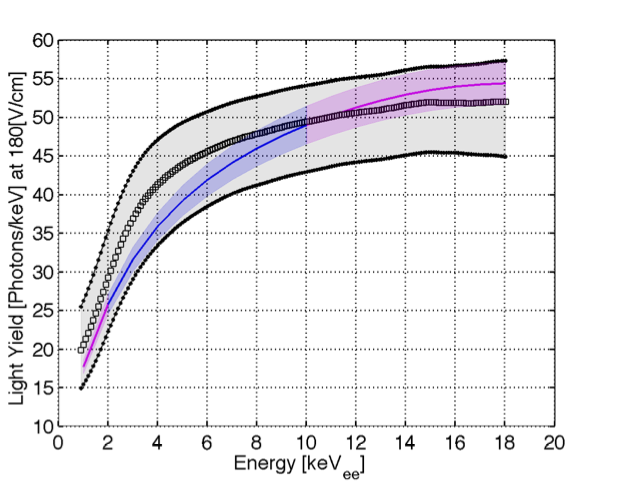
\includegraphics[width=73mm]{Chapter_Flucs/Figures/LYQY/LY_180_1sigBand_.png}}
\hfill
\subcaptionbox{$\rm n_e$, 170 V/cm \label{fig:5b}}{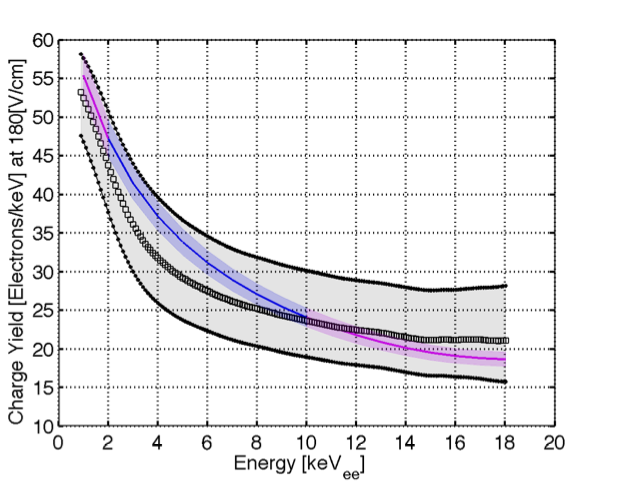
\includegraphics[width=73mm]{Chapter_Flucs/Figures/LYQY/QY_180_1sigBand_.png}}

\bigskip

\subcaptionbox{$\rm n_\gamma$ 100 V/cm \label{fig:5c}}{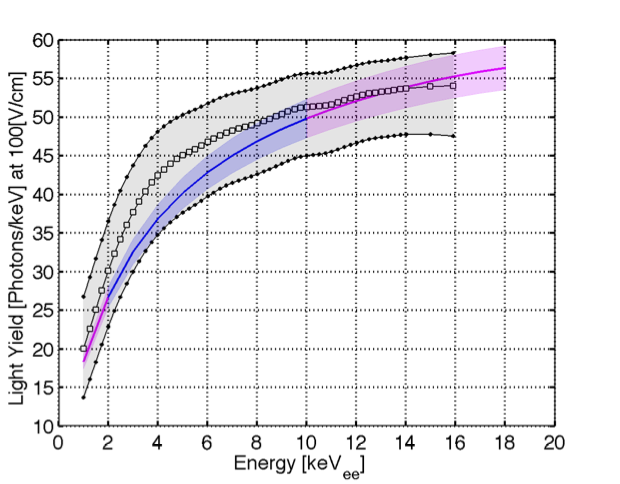
\includegraphics[width=73mm]{Chapter_Flucs/Figures/LYQY/LY_100_1sigBand_.png}}
\hfill
\subcaptionbox{$\rm n_e$, 100 V/cm \label{fig:5c}}{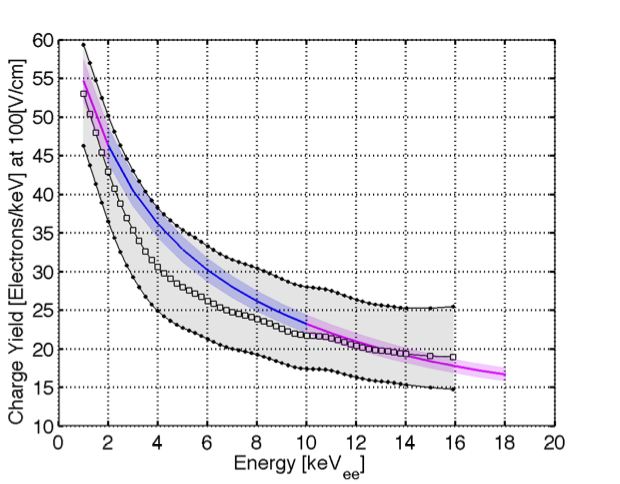
\includegraphics[width=73mm]{Chapter_Flucs/Figures/LYQY/QY_100_1sigBand_.png}}

\caption{Light yield and charge yield from tritium data without spectral shape correction at 180 [V/cm] in black, the shaded region represents the one sigma uncertainty on g1 and g2. The NEST yield prediction and it's corresponding 1 sigma is shaded in blue. NEST interpolation in show in magenta to energies where the model is not vetted. }
\label{fig:LYQY_iter0}
\end{figure}
\renewcommand{\baselinestretch}{2}
\small\normalsize


\newpage

\section{Measuring LY, QY, Recombination, Corrected for Spectral shape}

In the previous section we determined that the NEST model was not sufficient to produce a spectral shape correction for the tritium data. However, it was shown that and spectral shape correction is sufficiently small (less than 10\%) to extract light yield, charge yield and recombination from the tritium spectrum, using this information the model was improved and new simulations were produced. In this section we will take the information gathered in the previous section and apply the known detector resolution in order to create a spectral shape correction for the tritium S1 and S2. Having an improved model for NEST we can even determine the efficiency for  detecting tritium S1, S2 and the energy threshold, since the tritium spectrum still provides events well below the expected energy threshold of around 1.5 $\rm keV_{ee}$.


\subsection{Tritium S1 Correction}

Figure \ref{fig:S1_mapping_2} shows the application of smearing  from equation \ref{eq:S1_res} applied to the light yield extracted from the uncorrected tritium data with the data. The mapping for converting the observed S1 to the real S1 is shown in the figure. To calculate the correction we start with the extracted light yield, apply the measured g1, convolve it with a tritium beta spectrum and add in our first approximation of recombination fluctuations measured in equation \ref{eq:Inst_Fit}, given infinite detector resolution this is the spectrum the LUX detector would observe in S1 space. Knowing the dependance of detector resolution vs. the number of photons of a given event (equation \ref{eq:SigDet}) we can apply the model as outlined in \ref{sec:Smear} and calculate the shift from observed mean photons to real mean photons.

 \begin{figure}[h!]\centering
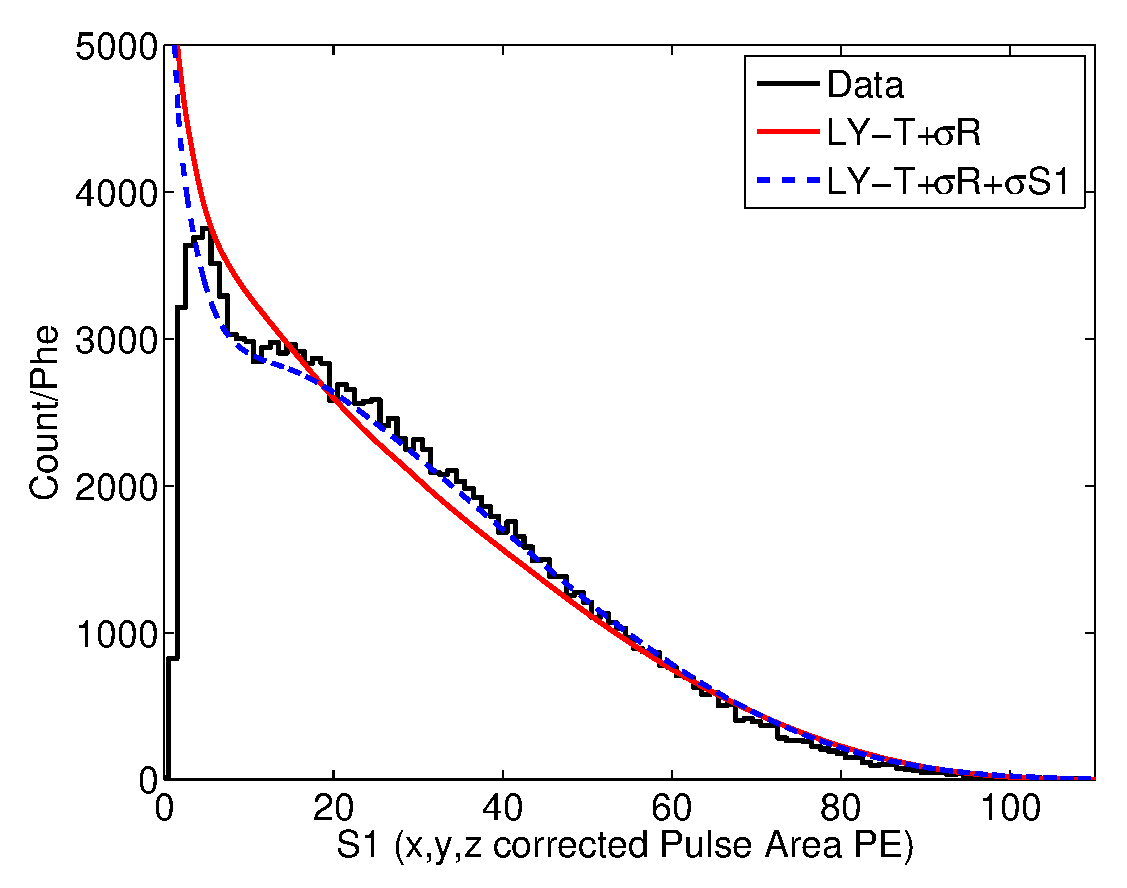
\includegraphics[width=70mm]{Chapter_Flucs/Figures/S1S2_Spectra/S1_spec_compare_iter1_.eps}
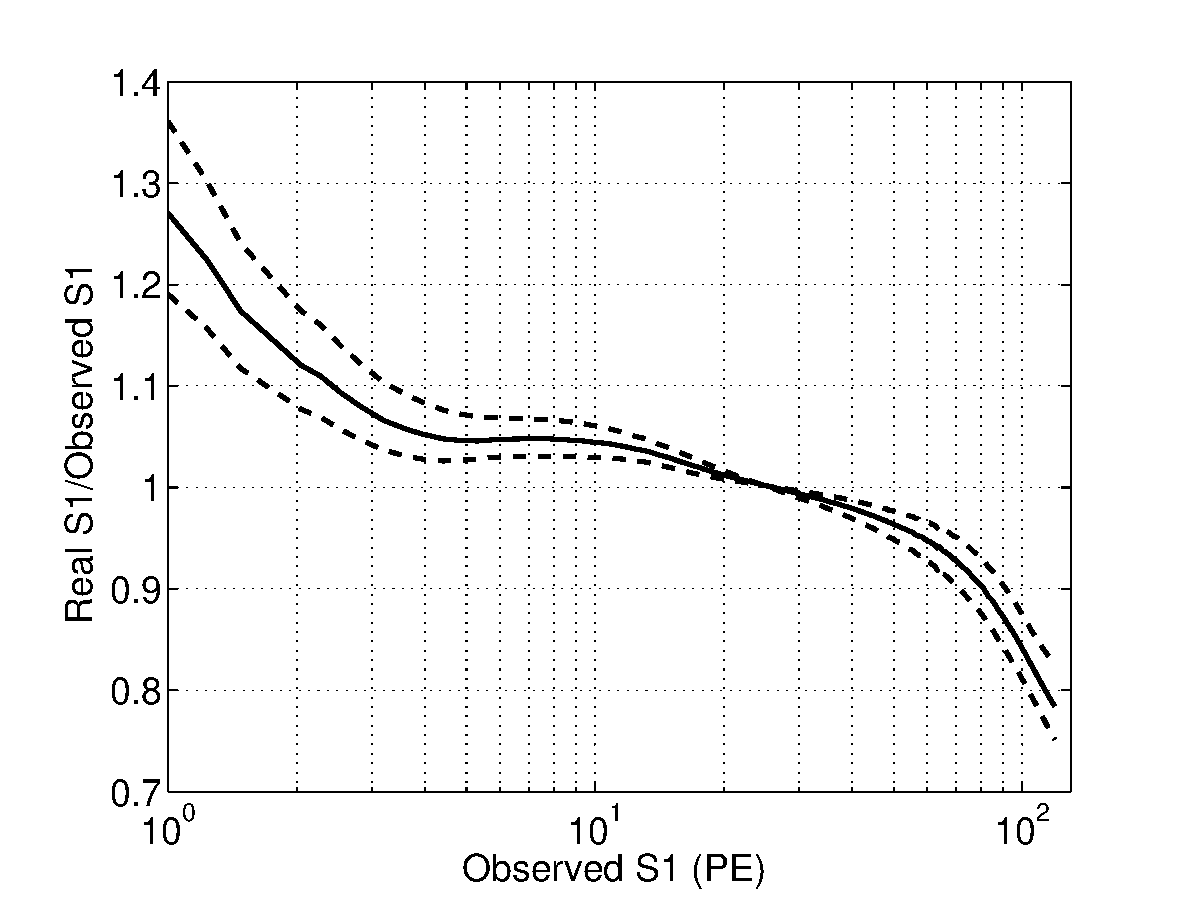
\includegraphics[width=70mm]{Chapter_Flucs/Figures/S1S2_Spectra/S1_corr_iter1_.eps}
\caption{Left: In Black, tritium data. In red, the spectrum after applying measured recombination fluctuations. In dashed blue is after applying recombination and finite detector resolution of equation. Left: Mapping of the observed mean, with finite resolution, to the mean with infinite resolution for a tritium photon spectrum. Bottom Right: The ratio of the real mean to the observed mean vs. the observed mean for a tritium photon spectrum. Note the S1 threshold at about 3 Phe in S1. }
\label{fig:S1_mapping_2}
\end{figure}

\subsection{Tritium S2 Correction}


Figure \ref{fig:S1_mapping_2} shows the application of smearing  from equation \ref{eq:S2_res} applied to the charge yield extracted from the uncorrected tritium data with the data. The mapping for converting the observed S2 to the real S2 is shown in the figure. To calculate the correction we start with the extracted light yield, apply the measured g2, convolve it with a tritium beta spectrum and add in our first approximation of recombination fluctuations measured in equation \ref{eq:Inst_Fit}, given infinite detector resolution this is the spectrum the LUX detector would observe in S1 space. Knowing the dependance of detector resolution vs. the number of electrons of a given event (equation \ref{eq:SigDet}) we can apply the model as outlined in \ref{sec:Smear} and calculate the shift from observed mean photons to real mean photons.

 \begin{figure}[h!]\centering
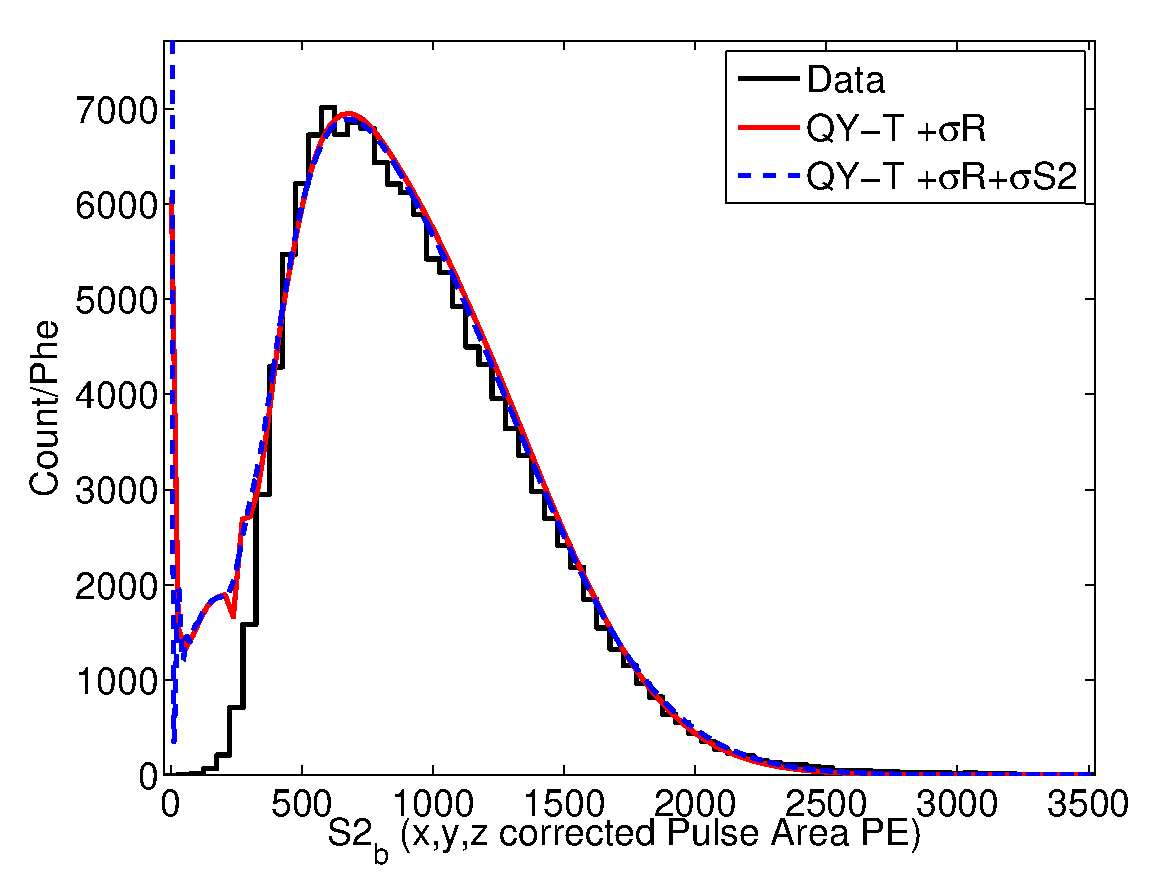
\includegraphics[width=70mm]{Chapter_Flucs/Figures/S1S2_Spectra/S2_spec_iter1_.eps}
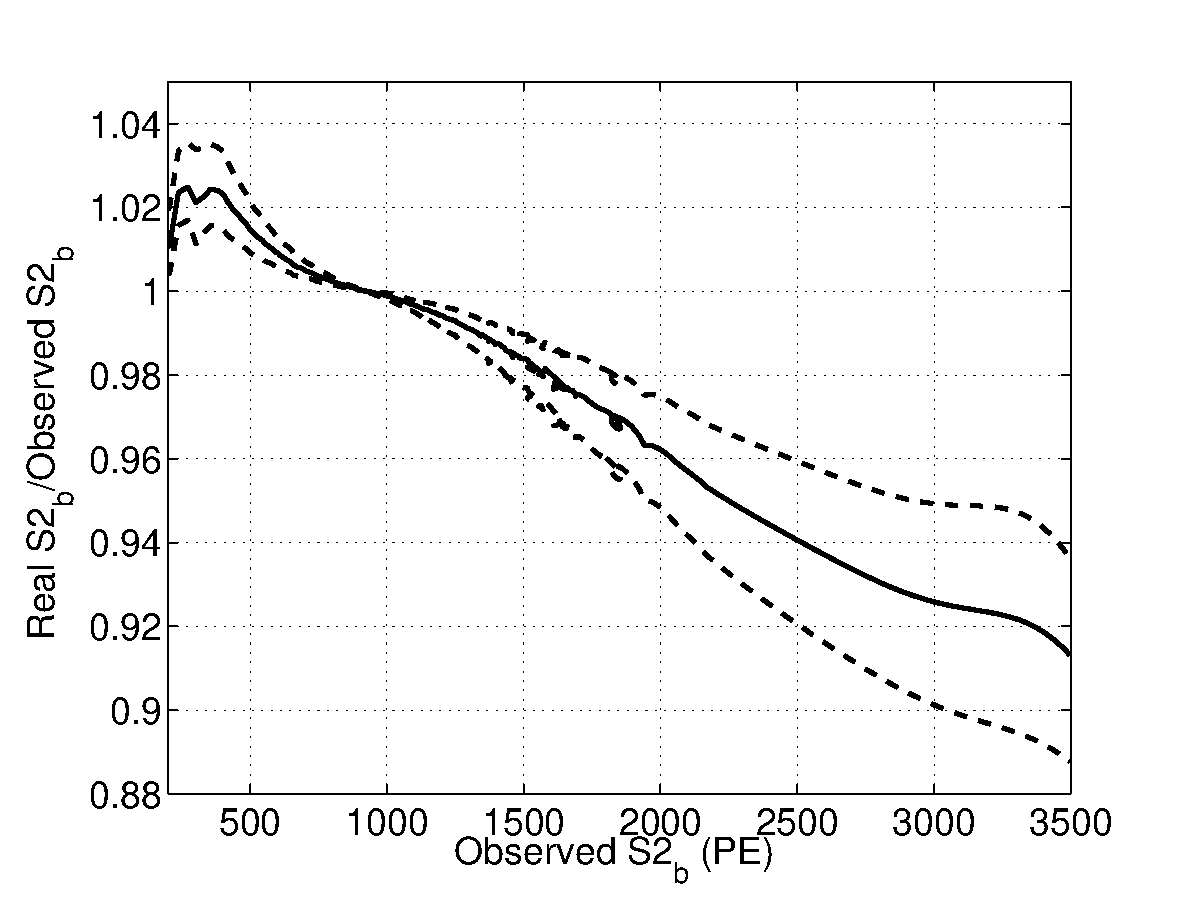
\includegraphics[width=70mm]{Chapter_Flucs/Figures/S1S2_Spectra/S2_corr_iter1_.eps}
\caption{Left: In Black, tritium data. In red, the spectrum after applying measured recombination fluctuations. In dashed blue is after applying recombination and finite detector resolution of equation. Left: Mapping of the observed mean, with finite resolution, to the mean with infinite resolution for a tritium photon spectrum. Bottom Right: The ratio of the real mean to the observed mean vs. the observed mean for a tritium photon spectrum. Note the S2 threshold at about 400  Phe. }
\label{fig:S2_mapping_2}
\end{figure}

\newpage

\section{Thresholds}

\begin{figure}[h!]\centering
 
\subcaptionbox{S1 \label{fig:3a}}{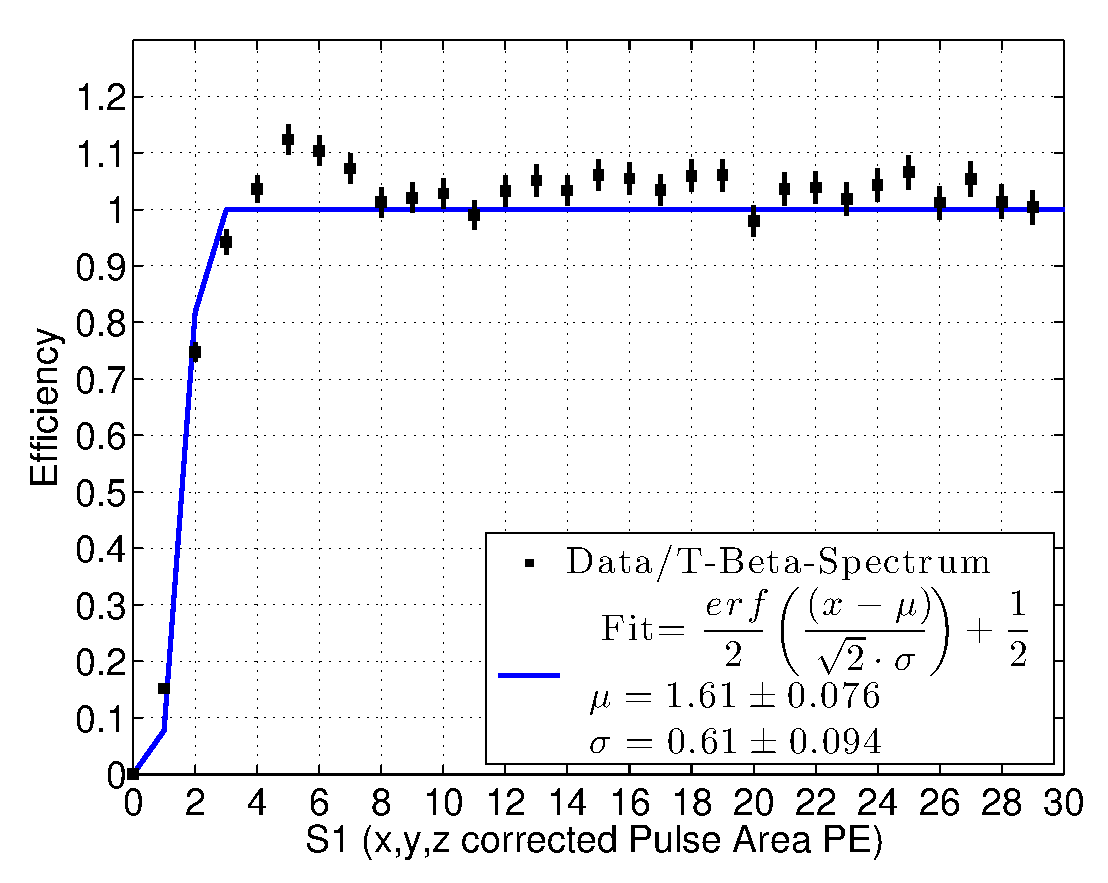
\includegraphics[width=70mm]{Chapter_Flucs/Figures/S1S2_Spectra/S1_Thres_.eps}}
\hfill
\subcaptionbox{$\rm S2_b$ (golden) \label{fig:3b}}{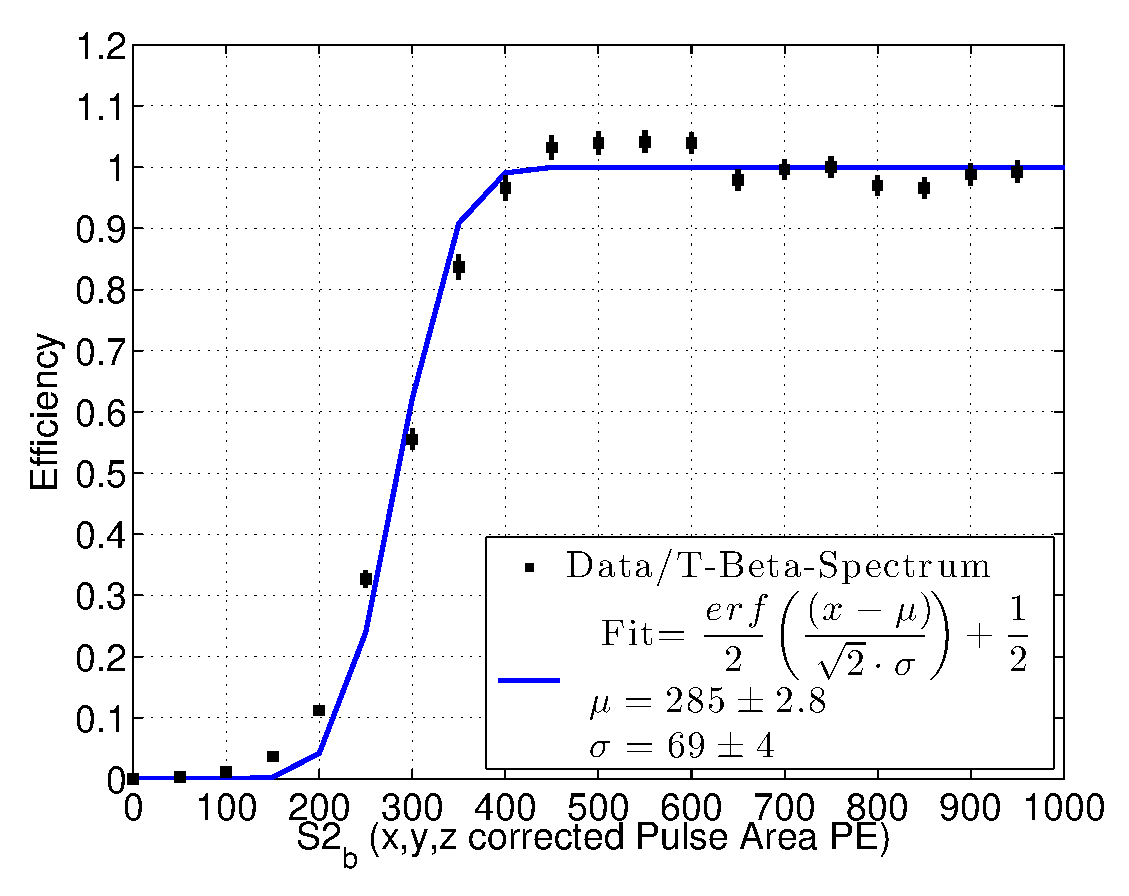
\includegraphics[width=70mm]{Chapter_Flucs/Figures/S1S2_Spectra/S2_Thres_.eps}}

\bigskip

\subcaptionbox{Combined Energy \label{fig:3c}}{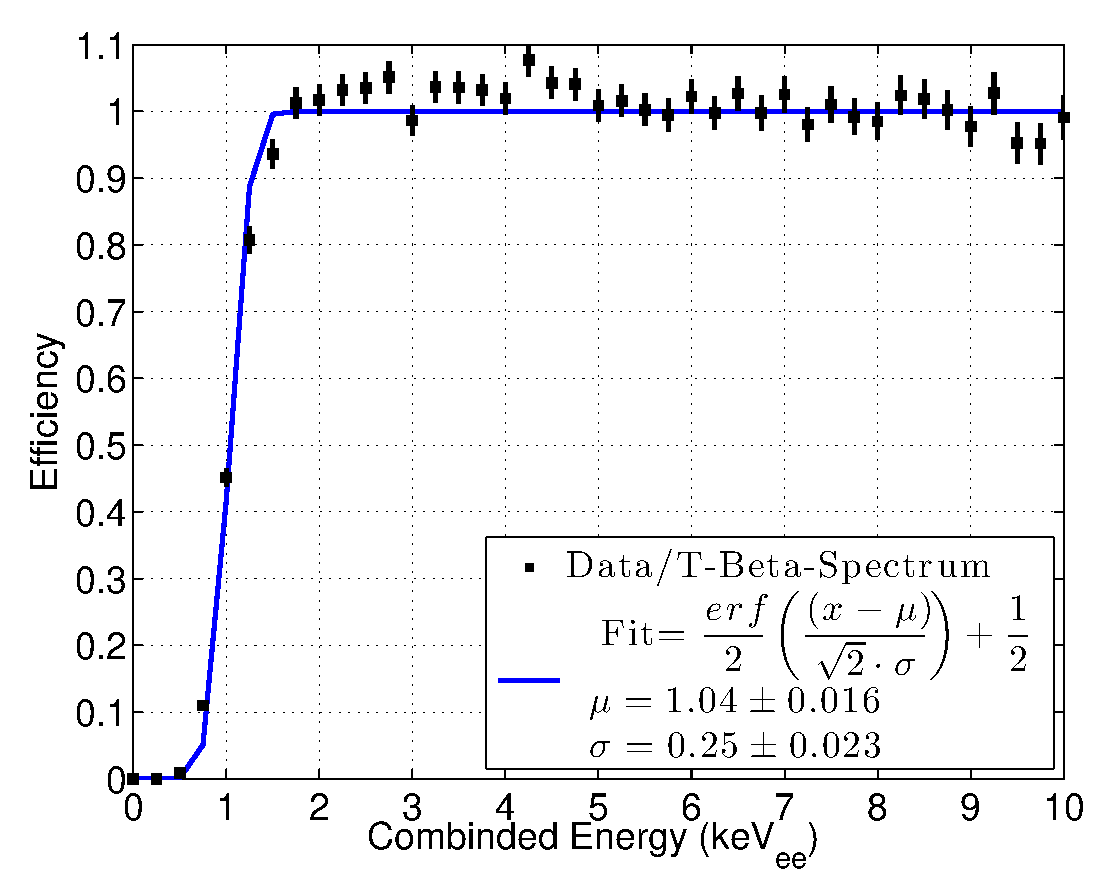
\includegraphics[width=70mm]{Chapter_Flucs/Figures/E_Spec/E_Thres_LY_QY_iter1.eps}}

\caption{Threshold calculated from difference of simulated Tritium S1, S2 and energy spectra. a) S1 b) $\rm S2_b$, c) Energy . The data set contained 140,000 tritium events in the fiducial}
\label{fig:Thres}
\end{figure}


\begin{figure}[h!]\centering
 
\subcaptionbox{S1 \label{fig:3a}}{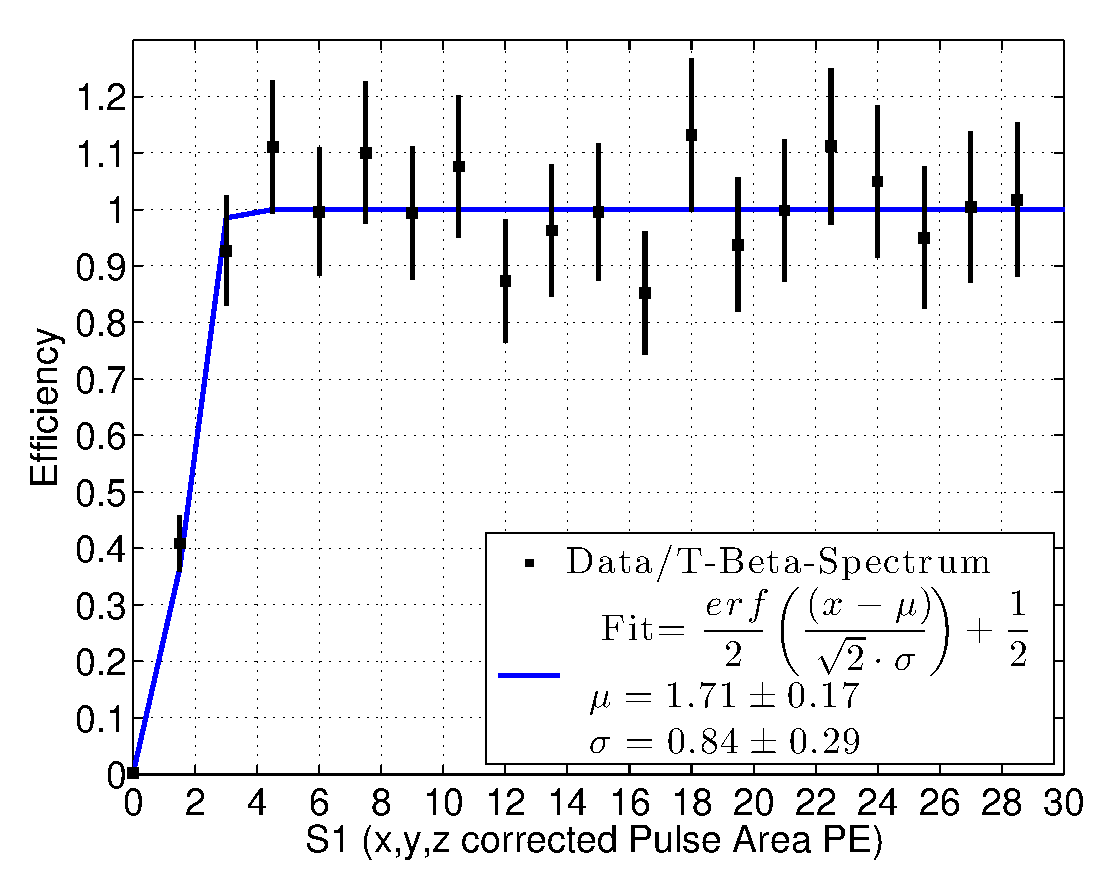
\includegraphics[width=70mm]{Chapter_Flucs/Figures/Spec_Thresh_100/S1_Thres_.eps}}
\hfill
\subcaptionbox{$\rm S2_b$ (golden) \label{fig:3b}}{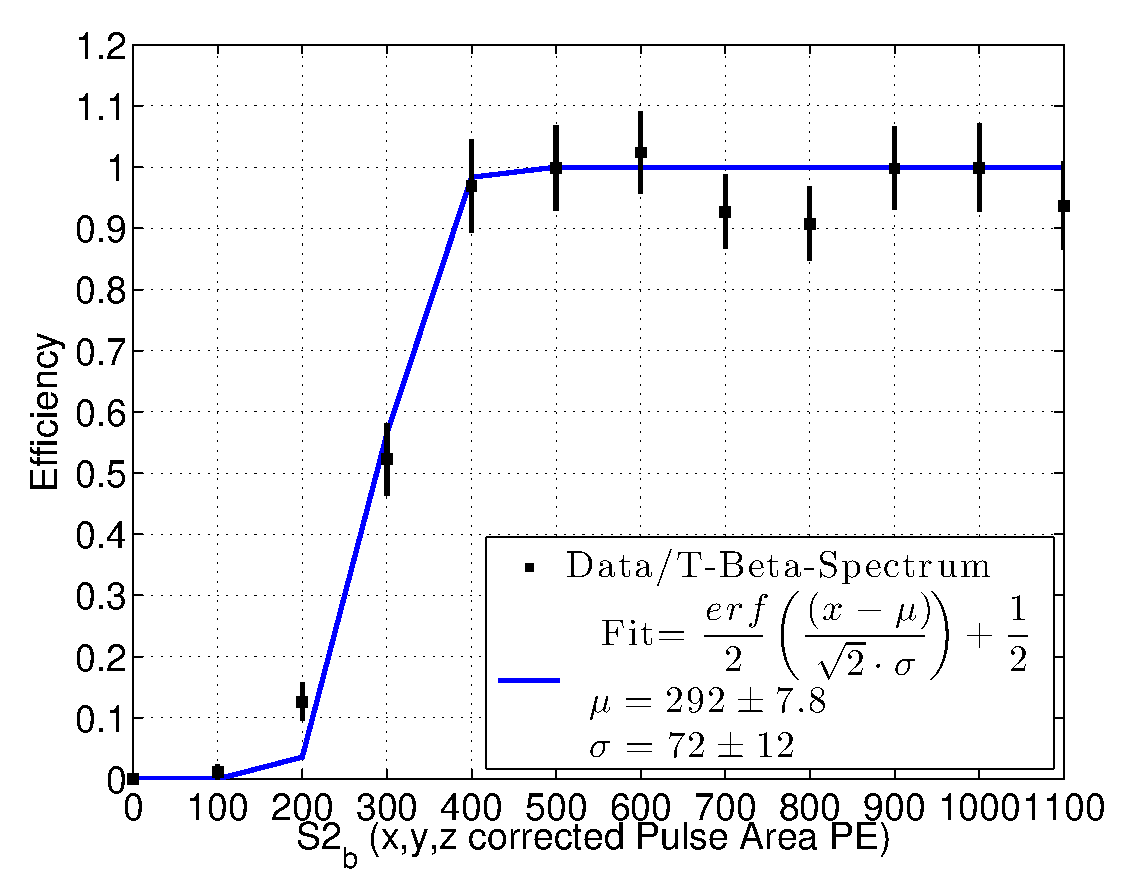
\includegraphics[width=70mm]{Chapter_Flucs/Figures/Spec_Thresh_100/S2_Thres_.eps}}

\bigskip

\subcaptionbox{Combined Energy \label{fig:3c}}{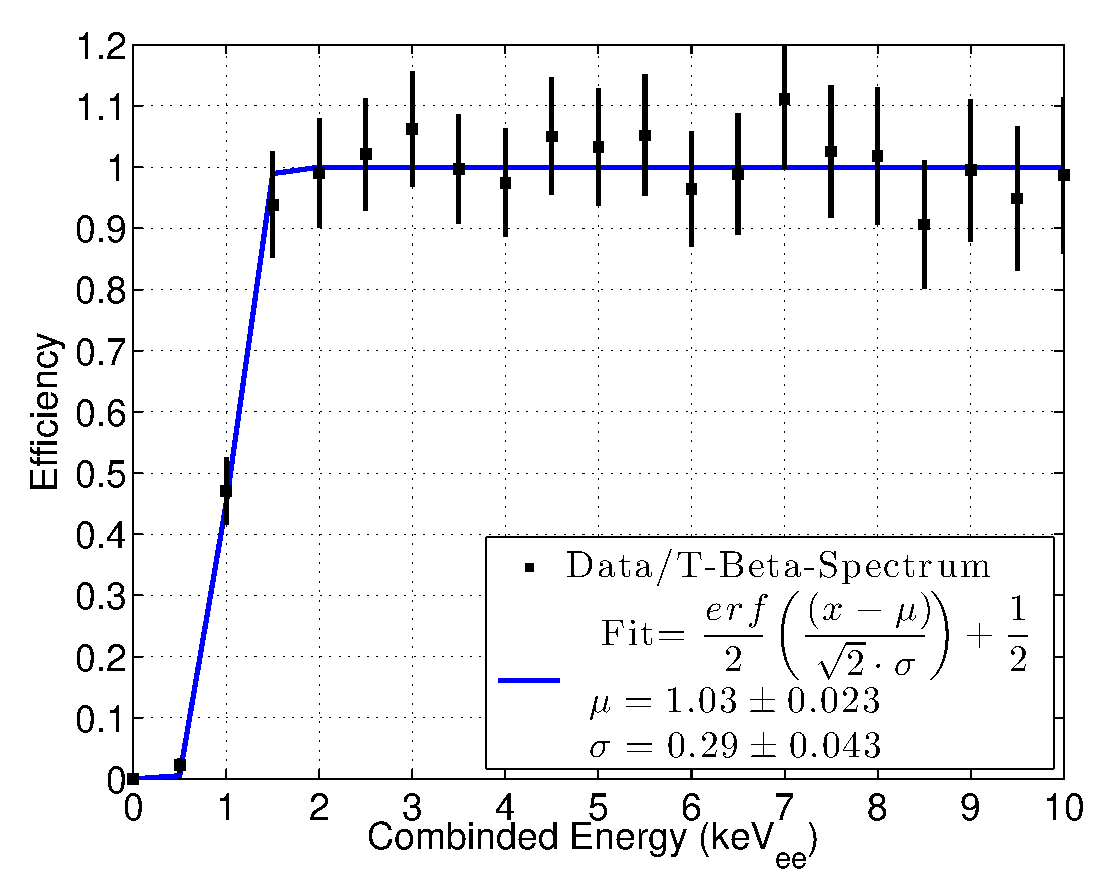
\includegraphics[width=70mm]{Chapter_Flucs/Figures/Spec_Thresh_100/E_Thres_.eps}}

\caption{Threshold calculated from difference of simulated Tritium S1, S2 and energy spectra at 100 V/cm. a) S1 b) $\rm S2_b$, c) Energy . The data set contained 2,500 tritium events in the fiducial.}
\label{fig:Thres_100}
\end{figure}


\newpage

\section{Ionization and Scintillation Yield After Correction}

 
\newpage


%LY QY and stat, raw data

\renewcommand{\baselinestretch}{1}
\small\normalsize
\begin{figure}[h!]\centering
 
\subcaptionbox{$\rm n_\gamma$, 170 V/cm \label{fig:5a}}{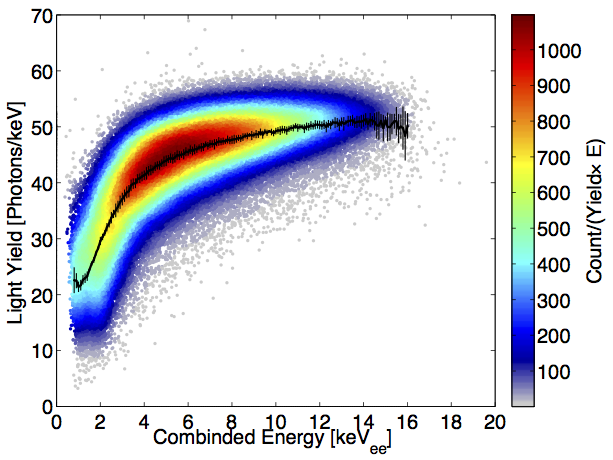
\includegraphics[width=73mm]{Chapter_Flucs/Figures/LYQY_Iter1/LY_c_180_means_.png}}
\hfill
\subcaptionbox{$\rm n_e$, 170 V/cm \label{fig:5b}}{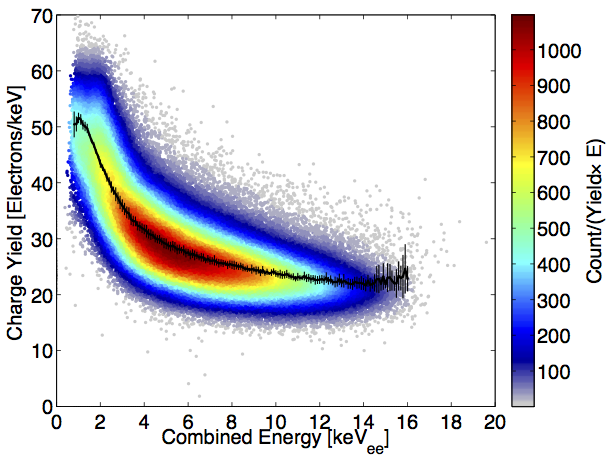
\includegraphics[width=73mm]{Chapter_Flucs/Figures/LYQY_Iter1/QY_c_180_means_.png}}

\bigskip

\subcaptionbox{$\rm n_\gamma$ 100 V/cm \label{fig:5c}}{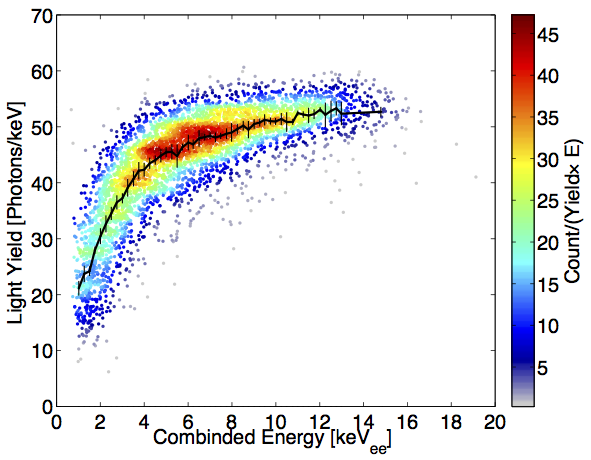
\includegraphics[width=73mm]{Chapter_Flucs/Figures/Iter1_100/LY_c_100_means_.png}}
\hfill
\subcaptionbox{$\rm n_e$, 100 V/cm \label{fig:5c}}{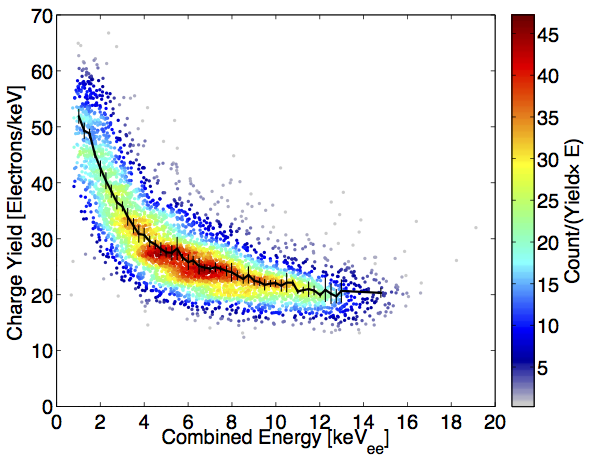
\includegraphics[width=73mm]{Chapter_Flucs/Figures/Iter1_100/QY_c_100_means_.png}}

\caption{LY and QY from tritium data corrected for spectral shape along with the 1 sigma band of g1/g2. The blue and magenta curve are NEST extrapolation and interpolation, respectively.}
\label{fig:LYQY_data}
\end{figure}
\renewcommand{\baselinestretch}{2}
\small\normalsize



%LY QY result

\renewcommand{\baselinestretch}{1}
\small\normalsize
\begin{figure}[h!]\centering
 
\subcaptionbox{$\rm n_\gamma$, 170 V/cm \label{fig:5a}}{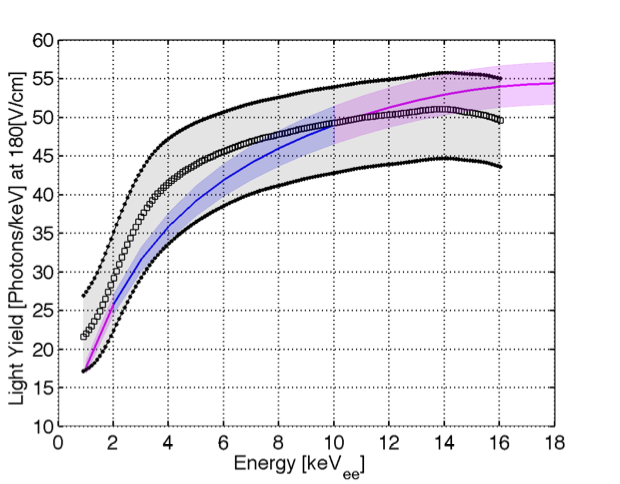
\includegraphics[width=73mm]{Chapter_Flucs/Figures/LYQY_iter1/LY_180_iter1_1sigBand_.png}}
\hfill
\subcaptionbox{$\rm n_e$, 170 V/cm \label{fig:5b}}{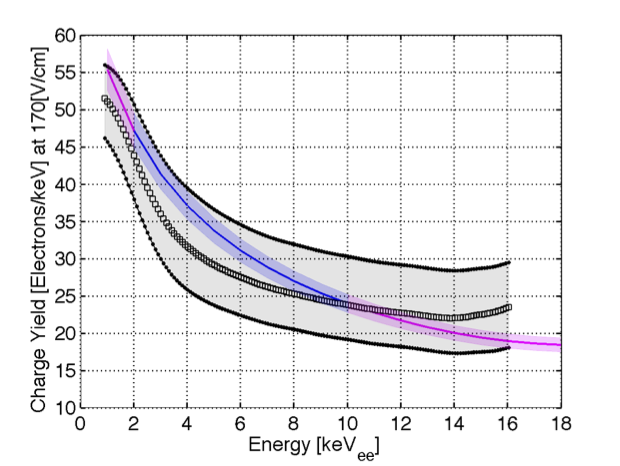
\includegraphics[width=73mm]{Chapter_Flucs/Figures/LYQY_iter1/QY_180_1sigBand_.png}}

\bigskip

\subcaptionbox{$\rm n_\gamma$ 100 V/cm \label{fig:5c}}{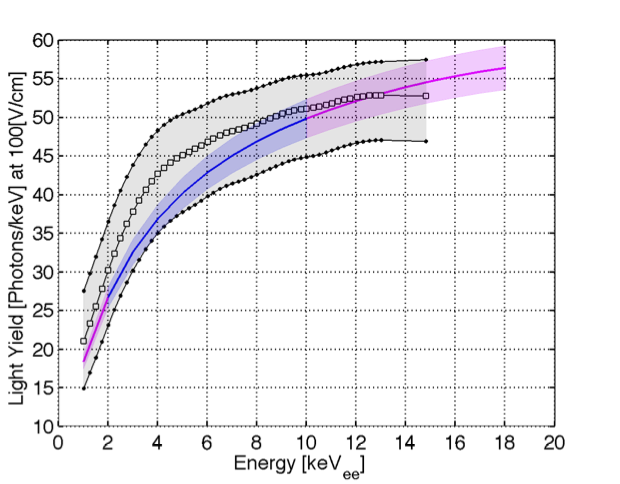
\includegraphics[width=73mm]{Chapter_Flucs/Figures/LYQY_iter1/LY_100_iter1_1sigBand_.png}}
\hfill
\subcaptionbox{$\rm n_e$, 100 V/cm \label{fig:5c}}{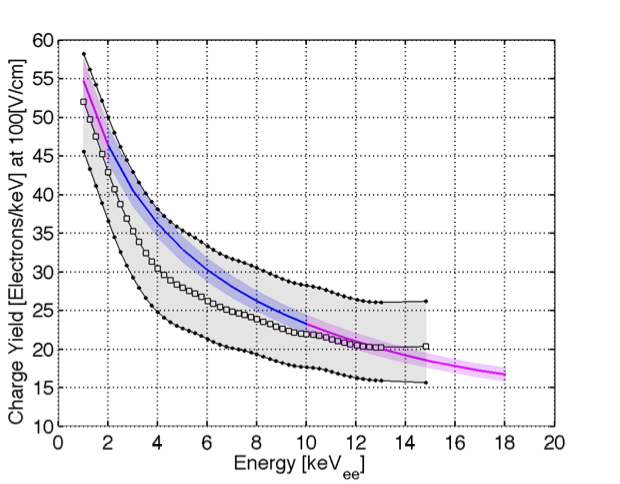
\includegraphics[width=73mm]{Chapter_Flucs/Figures/LYQY_iter1/QY_100_iter1_1sigBand_.png}}

\caption{LY and QY from tritium data corrected for spectral shape along with the 1 sigma band of g1/g2. The blue and magenta curve are NEST extrapolation and interpolation, respectively.}
\label{fig:LYQY_iter1}
\end{figure}
\renewcommand{\baselinestretch}{2}
\small\normalsize




 \begin{figure}[h!]\centering
 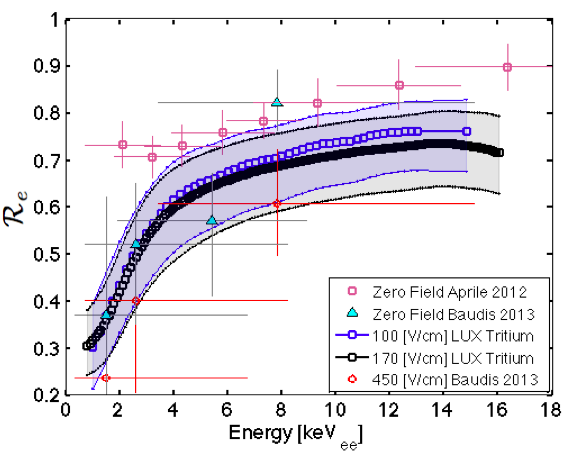
\includegraphics[width=140mm]{Chapter_Flucs/Figures/LYQY_iter1/Re_fig.png}
\caption{LY relative to the light yield of the 32.1 keV decay of \KrCal at zero field.}
\label{fig:LYQY_data}
\end{figure}

\newpage

\section{The Standard Candle. Light Yield from $\rm^{83m}Kr$}

Quenching of scintillation yield vs. field has been  typically defined relative to 32.1 keV decay of $\rm^{83m}Kr$ at zero field \cite{Aprile_LY},\cite{Baudis}. $\rm^{83m}Kr$ first emits a 32.1 [keV] gamma followed by a 9.4 [keV] with a half life of 154 [ns] between the two (refs). The combined signal (41.6 [keV]) is found by the pulse finder in the majority of cases, using the standard WIMP search pulse gap setting of 500 ns. However, the combined signal is not useful as a standard calibration since the light yield from the second 9.4 keV decay depends strongly on decay time separation. The second 9.4 keV decay is effected by the presence of exitons from the initial 32.1 [keV] decay. See figure [ show LUX result]

Fortunately, the first 32.1 keV appears to have no time dependance as it decays in `relaxed' xenon without the presence of additional exitons \cite{Aprile_LY}. For purposes of light yield normalization at zero field the 32.1 keV gamma serves as a good low energy standard candle for xenon detectors.

There were two data sets in late 2013 that contain $\rm^{83m}Kr$ decays at zero field. Since the S2 (charge) signal is unavailable the top-bottom asymmetry, $\frac{top-bottom}{top+bottom} $, is used to define the Z coordinate for position dependent corrections. The XY correction is subdominant to the Z dependent correction for light yield. Figure [] shows the linear mapping from top-bottom asymmetry to detector depth (Z). With the Z correction applied the average pulse area (Phe) normalized to the detector center (241.6 mm below the gate grid) is found to be $\rm 267.4 \pm^{stat} 1.5 \pm^{sys} 5$. See Figure \ref{fig:ZeroField_Kr}.

 
 \begin{figure}[h!]\centering
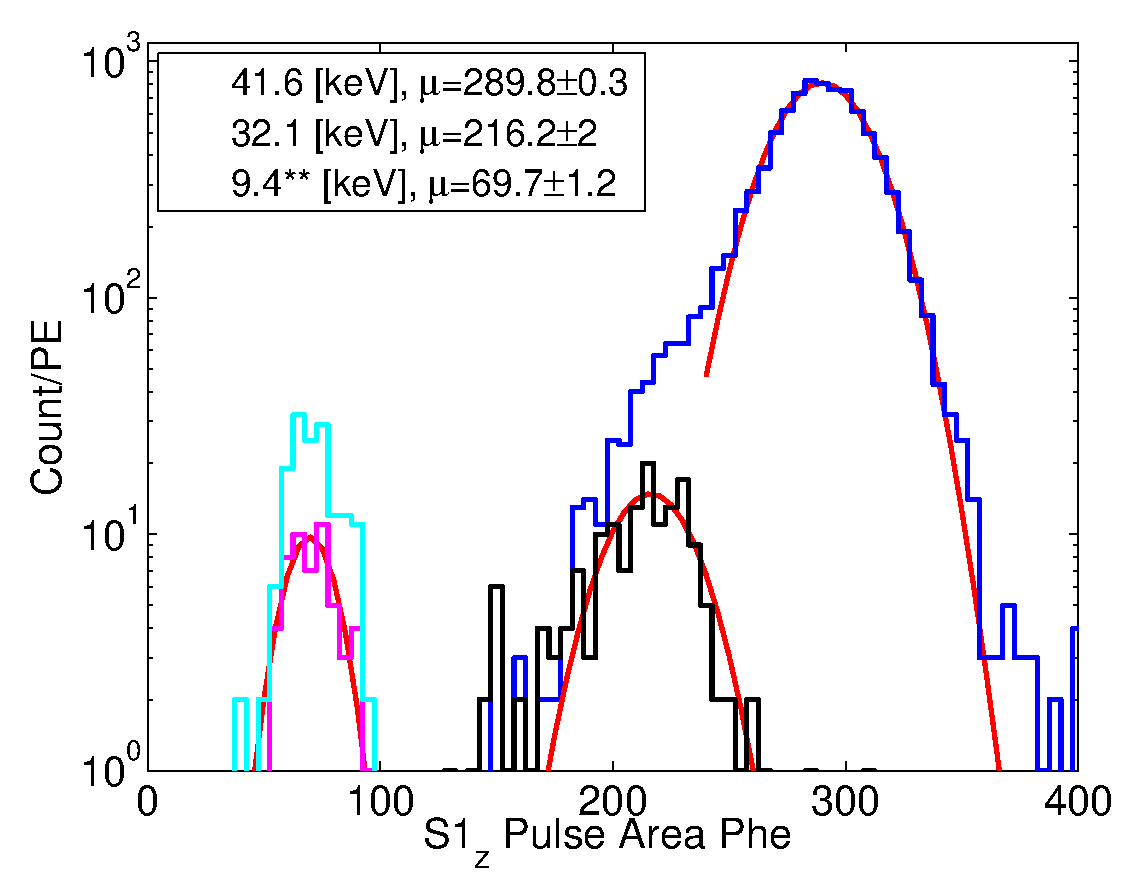
\includegraphics[width=72mm]{Chapter_Flucs/Figures/S1_Z_no_field_lux10_20131009T1358_cp09670} %old cp 6914
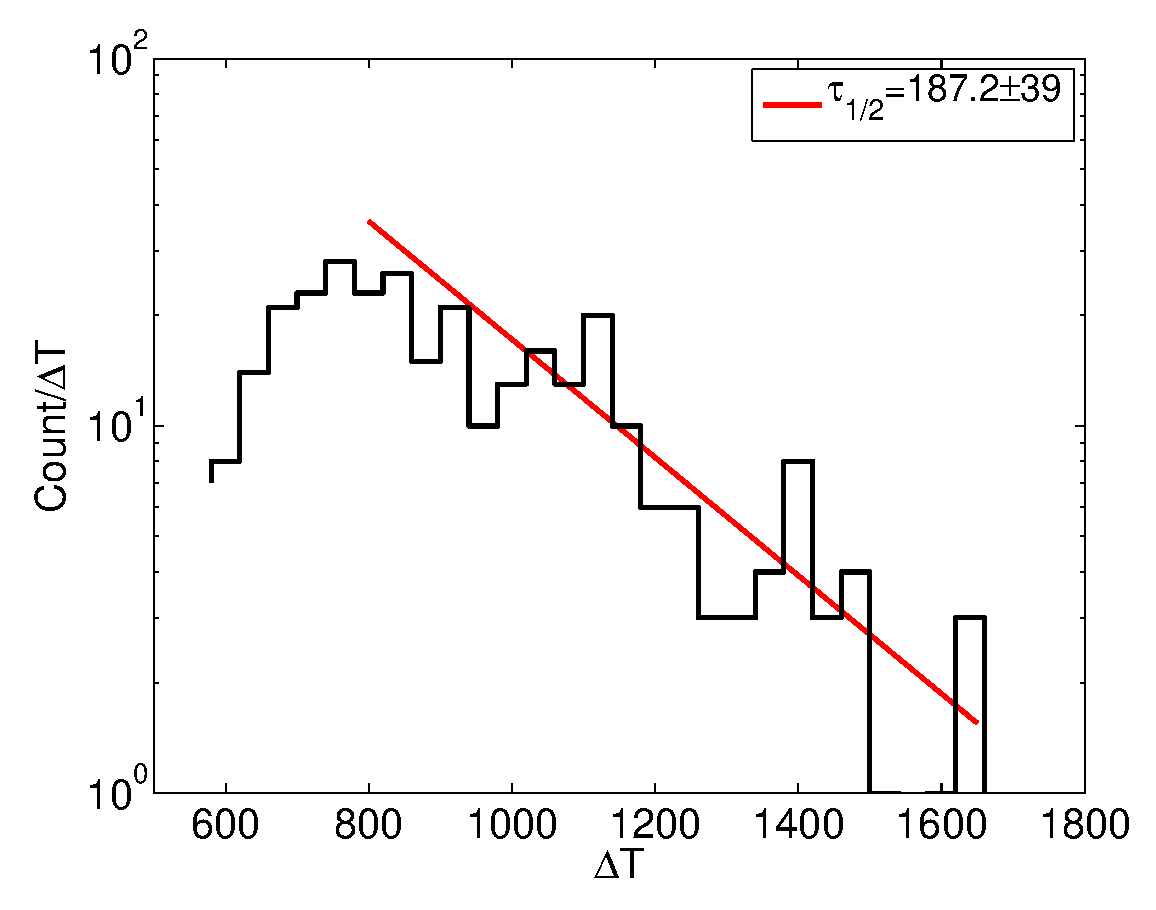
\includegraphics[width=72mm]{Chapter_Flucs/Figures/dT_no_field_2lux10_20131009T1358_cp09670}
\caption{Left: $\rm^{83m}Kr$ peaks at zero field. ** The 9.4 keV peak is fit only for events with a decay time separation greater than 1000 [ns]. Right: shows the timing separation between the 32.1 and 9.4 [keV] decays plotted above.}
\label{fig:ZeroField_Kr}
\end{figure}
 
\subsection{Field dependence of light yield from the 32.1 keV gamma of $\rm ^{83m}Kr$ }

Charge separation increases with drift field leading to less recombination for light production, causing scintillation yield to be quenched. See table \ref{table:kr32} for a list of the measured scintillation of the 32.1 keV gamma from $\rm ^{83m}Kr$, also includes the NEST predictions.

\renewcommand{\baselinestretch}{1}
\small\normalsize
\begin{table}[h!]
\begin{center}
\begin{tabular}{|c|c|c|c|c|c|}
\hline
Field	&S1			& Photons						& Yield 								&NEST	 \\
V/cm	& PE					& $\left<n_{\gamma}\right>$		& $\left<n_{\gamma}\right>$/keV	& $\left<n_{\gamma}\right>$/keV \\ \hline
0 		&	216.2 $\pm$ 5.0 	&2228.9 $\pm$ 50.5 &	69.4 $\pm$	1.6 	&	64.2 $\pm$ 3.2  \\ \hline
50 		&	195.0 $\pm$ 0.7 	&2010.3 $\pm$ 7.2   & 	62.6 $\pm$	0.2	&	59.8 $\pm$ 3.0 \\ \hline
100 	&	178.4 $\pm$ 0.7 	&1839.2 $\pm$ 	7.2	 &	57.3 $\pm$ 0.2 	&	55.8 $\pm$ 2.8 \\ \hline
170 	&  171.4 $\pm$ 0.9		&1767.0 $\pm$ 	9.2  &	55.0 $\pm$ 0.3 	&	51.9 $\pm$ 2.6 \\ \hline
\end{tabular}
\caption{Field dependance of the light yield form the 32.1 keV decay of $\rm^{83m}Kr$. The fields are calculated using a two dimensional model and not accounting potential charge accumulation on inner teflon panels.}
\label{table:kr32}
\end{center}
\end{table}
\renewcommand{\baselinestretch}{2}
\small\normalsize



%\begin{table}[h!]
%\begin{center}
%\begin{tabular}{|c|c|c|c|c|c|c|}
%\hline
%Field 	&41.6 [keV] 	& 32.1 [keV] 	& 9.4* [keV] 	&9.4** [keV] & S2	&S2 ** \\ 
% \[[V/cm]	&	S1PE	&S1PE	&S1PE&		S1PE		&S2PE		&S1PE  \\ \hline
%0 	&		359.9 $\pm$ 5	 			&267.4 $\pm$ 6.5 		&78 $\pm$ 2	 	&	 92.5$\pm$	6 		&	--  			& --	\\ \hline
%51 &		332.6 $\pm$ 1.4 			&246.7 $\pm$ 1.2 		&76.4 $\pm$ 0.5 	& 	86 $\pm$ 1		 &	3651 $\pm$ 5	& 3708 $\pm$ 11 \\ \hline
%105 &		316.8 $\pm$ 1.4 			&233.6 $\pm$ 1.4 		&72.9$\pm$ 0.5		 &	83 $\pm$ 1 			&	4357 $\pm$ &4399 $\pm$ 16 \\ \hline
%182	 & 		291.3 $\pm$ 1.4 			&212.3 $\pm$ 1.3		&68.8 $\pm$ 0.5 	&	79 $\pm$ 1 		&	4986 $\pm$ 5 	 &5048$\pm$ 13 \\ \hline
%\end{tabular}
%\caption{Field dependance of the light yield form the 32.1, 9.4 and combined 41.6 [keV] decay of $\rm^{83m}Kr$. The fields are calculated using a two dimensional model and not accounting potential charge accumulation on inner teflon panels. ** *}
%\end{center}
%\label{table:krAll}
%\end{table}